% !TEX program = xelatex
\documentclass[aspectratio=169]{beamer}
\usepackage{tikz}
\usepackage{tikz-cd}
\usepackage{quiver}
\usepackage{calc}
\usefonttheme[onlymath]{serif}
\usepackage{polyglossia}
\setmainlanguage{vietnamese}
\usepackage[outputdir=out]{minted}
\usepackage{amsthm,amsmath,amssymb}
\newtheorem{thm}{Định lý}
\newtheorem{defn}{Định nghĩa}
\usepackage{caption}
\usepackage{subcaption}
\usepackage{graphicx}
\usepackage{float}
\usepackage{cancel}
\usepackage{mathtools}

\setbeamertemplate{theorems}[numbered]

\setbeamerfont{footnote}{size=\tiny}
%% TYPESET
\makeatletter
\newcommand{\leqnomode}{\tagsleft@true}
\newcommand{\reqnomode}{\tagsleft@false}
\makeatother
\newcommand{\norm}[1]{\left\lVert#1\right\rVert}
\newcommand{\abs}[1]{\left\lvert#1\right\rvert}
\newcommand{\gr}{\operatorname{gr}}
\newcommand{\rank}{\operatorname{rank}}
\newcommand{\toto}{\rightrightarrows}%
\newcommand{\F}{\Mathcal{F}}%
\newcommand{\K}{\mathbb{K}}%
\newcommand{\R}{\mathbb{R}}%
\def\C{\mathbb{C}}%
\newcommand{\dom}{\operatorname{dom}}%
\newcommand{\im}{\operatorname{im}}%
\newcommand{\g}{\mathcal{g}}%
\global\long\def\MP{\text{mp}}%

\newcommand{\Image}[1]{%
	\sbox0{\includegraphics[height=0.65\paperheight]{#1}}%
	\ifdim\wd0 < \textwidth
	\includegraphics[height=0.65\paperheight]{#1}%
	\else
	\includegraphics[width=\textwidth]{#1}%
	\fi%
}

\newif\iffirsttoc
\firsttoctrue
\AtBeginSubsection[]
{
  \parskip=0pt
  \begin{frame}[allowframebreaks]
        \frametitle{Mục lục}  
        \iffirsttoc
            \tableofcontents
            \global\firsttocfalse
        \else
            \tableofcontents[currentsection,
            % hideothersubsections,
            subsectionstyle=show/shaded/hide,
            subsubsectionstyle=show/show/show/hide
            ]
        \fi
    \end{frame} 
  \parskip=1em
}
\setbeamertemplate{caption}[numbered]

% \usetheme{hust}
% \titlegraphic{\includegraphics[height=\logoheight]{figures/sami-v2.pdf}}
\title{Báo cáo}
% \subtitle{\textbf{\LARGE Tìm bán kính điều khiển có cấu trúc của hệ chịu\\đa nhiễu sử dụng các toán tử tuyến tính đa trị}}
\subtitle{\textbf{Các thuật toán cơ bản của Tiến hóa Đa nhiệm
    \\(Evolutionary Multi-Task Optimization)}}

\author{Nhóm 1 - CTTN Khoa học Máy tính K67}
\iffalse
{Nguyễn Văn An - ...\\Ngô Duy Anh - 20200069\\Nguyễn Anh Bảo - \\Đặng
Tiến Cường - a}
\fi
\date{Tháng 1, 2024}

\begin{document}
\begin{frame}[noframenumbering]
	\titlepage
\end{frame}

\section{Ứng dụng các cơ chế tiến hóa trong tối ưu} % (fold)
\label{sec:Ứng dụng các cơ chế tiến hóa trong tối ưu}

\subsection{Chọn lọc tự nhiên và Thuyết tiến hóa của C. Darwin} % (fold)
\label{sub:Chọn lọc tự nhiên và Thuyết tiến hóa của C. Darwin}

\begin{frame}{Chọn lọc tự nhiên và Thuyết tiến hóa của C. Darwin}
Gần 4 tỉ năm trước, sự sống xuất hiện trên Trái Đất. Sau một khoảng thời gian
ấy, sự sống đã len lỏi đến mọi ngóc ngách của địa cầu, mang đủ loại hình thù từ
đơn giản đến phức tạp. Các nhà sinh học, sau khi nhìn thấy sự đa dạng này, đặt
ra câu hỏi rằng: tại sao các quy luật của tự nhiên, dường như ưa thích sự hỗn
loạn và thiếu trật tự, lại có thể tạo ra những loại tổ chức vật chất phức tạp và
dường như có chủ ý này.

Cho đến ngày nay, câu hỏi này vẫn chưa có một lời giải thích thỏa đáng. Tuy
nhiên, \textbf{Thuyết Tiến hóa} của C. Darwin đã, mặc dù có nhiều lỗ hổng, đã
trả lời được câu hỏi này một cách tương đối hoàn thiện.
\end{frame}

\begin{frame}{Chọn lọc tự nhiên và Thuyết tiến hóa của C. Darwin}
\begin{figure}
  \centering
  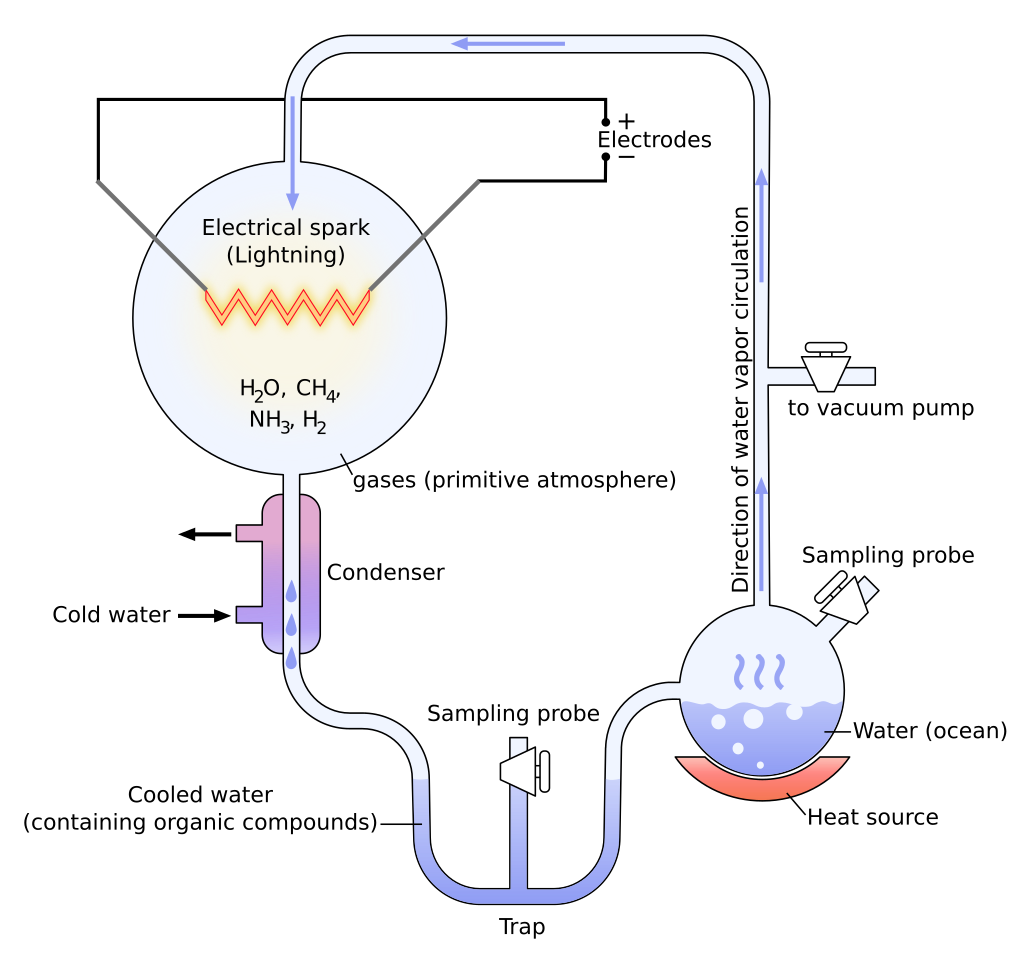
\includegraphics[width=0.8\textwidth, height=0.7\textheight,
  keepaspectratio]{res/miller-urey.png}
\captionsetup{justification=centering,margin=3cm}
  \caption{Thí nghiệm Miller-Urey, một thí nghiệm thất bại trong việc giải thích nguồn
  gốc của sự sống.}
\end{figure}
\end{frame}

\begin{frame}{Chọn lọc tự nhiên và Thuyết tiến hóa của C. Darwin}
Thuyết tiến hóa của C. Darwin đề cao một quá trình xảy ra trong tự nhiên:
\textbf{Chọn lọc tự nhiên}, coi đây là yếu tố quan trọng nhất sản sinh ra mọi
loài sinh vật.

Theo C. Darwin, để chọn lọc tự nhiên hoạt động như những gì xảy ra trong thực tế,
cần có ba điều kiện sau:

\begin{itemize}
\item Tính kế thừa (Heredity): Cần có một cách nào đó để chuyển giao các tính
  trạng từ cá thể cha mẹ sang các cá thể đời con.
\item Tính đa dạng (Variation): Trong hệ sinh thái, các cá thể cần có nhiều đặc
  điểm khác nhau, hoặc một cách để tạo ra các cá thể biến thể có đặc điểm khác
  với quần thể.
\item Tính chọn lọc (Selection): Phải có một phương thức nào đó mà một số cá thể
  trong quần thể được trở thành cá thể cha mẹ và sinh sản ra các thế hệ
  con, trong khi các cá thể khác không được hưởng quyền lợi này.
\end{itemize}
\end{frame}

% subsection Chọn lọc tự nhiên và Thuyết tiến hóa của C. Darwin (end)

\subsection{Giải thuật tiến hóa (Evolutionary Algorithms)} % (fold)
\label{sub:Giải thuật tiến hóa (Evolutionary Algorithms)}

\begin{frame}{Giải thuật tiến hóa (Evolutionary Algorithms)}
Trong tự nhiên, nhiều yếu tố tưởng chừng là ngẫu nhiên nhưng không phải. Chẳng
hạn, việc loài ong xây tổ có hình lục giác là do đây là hình đa giác có khả năng
lấp kín không gian (khác với hình tròn, hình ngũ giác), mà tiết kiệm được tối đa
lượng vật liệu để xây tổ.

Đây là do quá trình sinh sống của các cá thể trong tự nhiên có thể coi là một
bài toán tối ưu: tối ưu khả năng sinh tồn và sinh sản. Nói cách khác, đây chính
là độ \textbf{khỏe mạnh} (fitness) của cá thể.

\begin{figure}
\centering 
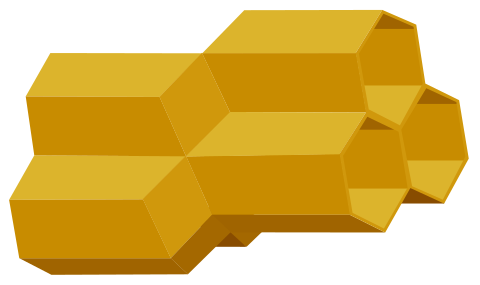
\includegraphics[width=\textwidth, height=0.2\textheight, keepaspectratio]
{res/honeycomb.png}
\caption{Dạng hình học của các ô tổ ong.}
\end{figure}
\end{frame}

\begin{frame}{Giải thuật tiến hóa (Evolutionary Algorithms)}
  Trước đây, con người huấn luyện các loài động vật thông qua thưởng hoặc
phạt, một việc làm ảnh hưởng trực tiếp đến độ khoẻ mạnh của cá thể, nhưng nếu
như bây giờ, ta có thể làm quá trình này hiệu quả hơn rất nhiều: bằng cách
\textbf{mô phỏng} lại quá trình này trong máy tính.

  Tuy nhiên, chúng ta không thể làm một mô phỏng chính xác 100\%
như với thực tế, mà chỉ có thể \textbf{chọn lọc các tính năng muốn mô phỏng}, và
\textbf{thực hiện các phép xấp xỉ phù hợp}. Mỗi cách này cho ta một thuật toán,
nằm trong lớp các \textbf{giải thuật tiến hóa}.

\begin{figure}
  \centering
  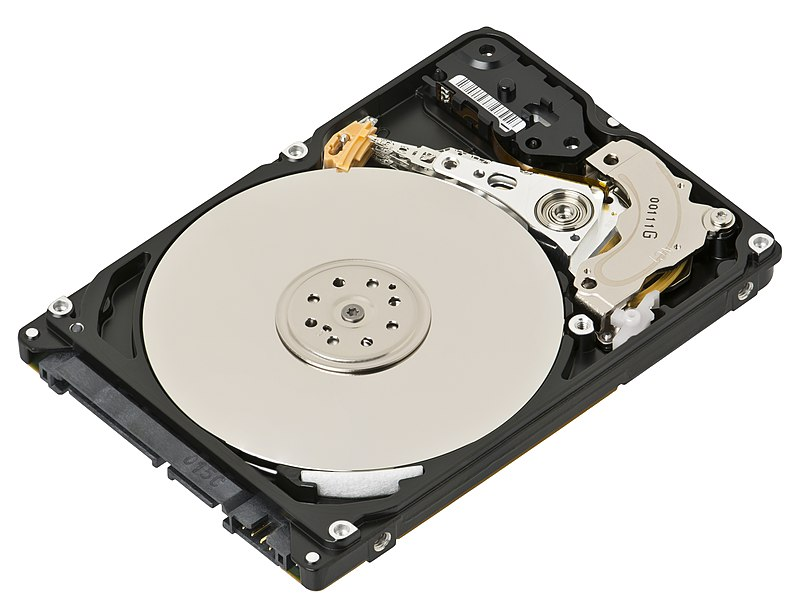
\includegraphics[width=0.8\textwidth, height=0.2\textheight,
  keepaspectratio]{res/hdd.jpg}
\captionsetup{justification=centering,margin=2.5cm}
  \caption{Người ta ước tính, để lưu lượng thông tin của
  các nguyên tử trong một ổ đĩa sẽ cần $10^{12}$ ổ đĩa như thế.}
\end{figure}
\end{frame}

% subsection Giải thuật tiến hóa (Evolutionary Algorithms) (end)

\subsection{Các khái niệm chung của các giải thuật tiến hóa} % (fold)
\label{sub:Các khái niệm chung của các giải thuật tiến hóa}

\begin{frame}{Hàm fitness và hàm mục tiêu}
Như đã nói ở phần trên, các giải thuật tiến hóa thực hiện mô phỏng lại quá trình
sống của các cá thể có trong tự nhiên. Các cá thể sẽ, một cách tự nhiên, 
sinh sản và tạo ra các cá thể khỏe mạnh hơn, và nhờ đó tiến hóa.

Do vậy, nếu ta đánh giá sự khỏe mạnh của một cá thể bằng một ánh xạ $f: P \to
\mathbb{R}$, từ $P$: tập các cá thể hợp lệ cho đến tập số thực, thì quá
trình trên sẽ làm tiến hóa các cá thể của nó làm tối đa $f$, giúp cho người dùng
thu được một nghiệm (có thể) tối ưu của hàm mục tiêu $f$.

$f$ ở đây, ngoài cách gọi là hàm mục tiêu (objective function) trong Toán tối ưu
(Mathemetical Optimization), trong các giải thuật tiến hóa còn được gọi là "hàm
độ khỏe mạnh"\footnote
{Thuật ngữ này không được sử dụng nhiều trong tiềng Việt,
nhưng thuật ngữ tương ứng trong tiếng Anh được sử dụng tương đối nhiều.} hay 
\textbf{hàm fitness} (fitness function), do tính liên quan mật thiết giữa $f$
với độ khoẻ mạnh của cá thể.

\end{frame}

\begin{frame}{Hàm fitness và hàm mục tiêu}
Giữa toán tối ưu và giải thuật tiến hóa có một sự bất đồng nho nhỏ như sau: các
bài toán tối ưu thường được phát biểu dưới dạng bài toán min, nhưng các giải
thuật tiến hóa sẽ làm tối đa hàm fitness. Do đó, có nhiều trường hợp mà ta không
tối đa hóa hàm fitness mà lại tối thiểu hóa nó.

\begin{figure}
\centering
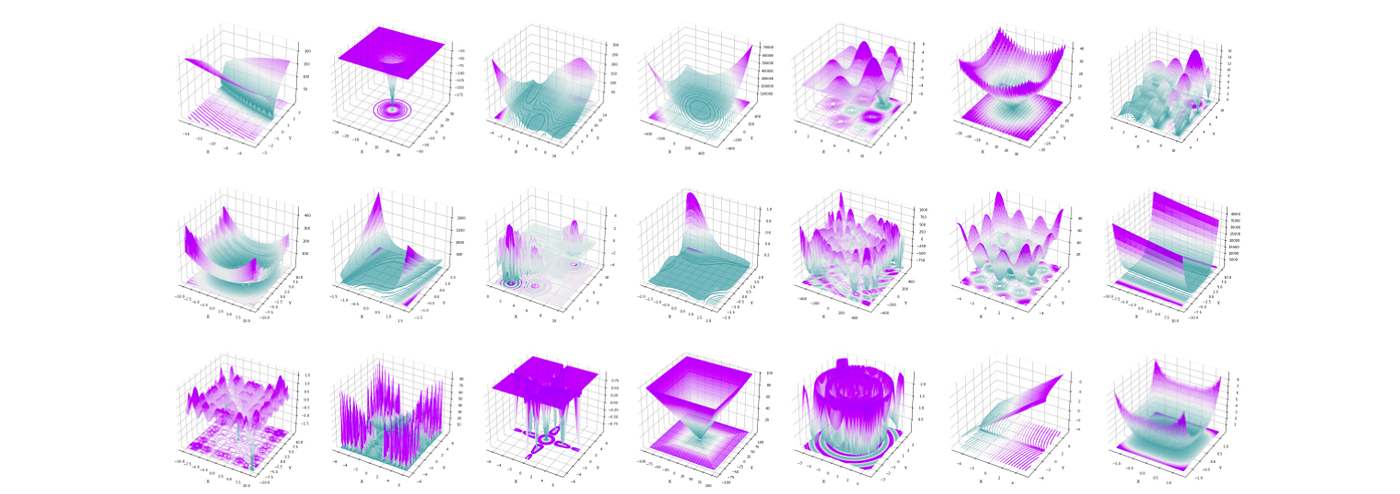
\includegraphics[width=\textwidth, height=0.5\textheight, keepaspectratio]
{res/discrep.png}
\captionsetup{justification=centering,margin=3cm}
\caption{Đồ thị hàm mục tiêu của các bài toán thử, thường được phát biểu dưới
dạng bài toán tìm min.}
\end{figure}
\end{frame}

\begin{frame}{Mã hóa cá thể}
Ở phần này, ta sẽ làm rõ hơn về cá thể. Về lý thuyết, cá thể trong giải thuật
tiến hóa có thể là bất cứ thứ gì, miễn là nó có khả năng sinh sản.

Tuy nhiên, lấy ý tưởng từ cách thông tin di truyền được lưu trữ trong ADN của
sinh vật dưới dạng hai chuỗi các nucleotide, người ta thường lấy dạng biểu diễn
của một ADN là một mảng kích thước định sẵn, thường là một mảng số nguyên hoặc
một mảng số thực. Mảng này được gọi là một \textbf{nhiễm sắc thể} (chromosome),
và các phần tử của nó là các \textbf{gen} (gene).

Vì thế, nảy sinh ra một vấn đề: ta cần một cách \textbf{mã hóa} một cá thể bất
kì: từ $P$ - tập các cá thể, sang $C$ - tập các nhiễm sắc thể, và ngược lại:
\begin{align*}
  \operatorname{encode}&: P \to C \\
  \operatorname{decode} &: C \to P \\
.\end{align*}
\end{frame}


\begin{frame}[fragile]
\frametitle{Mã hóa cá thể}
Với cá thể là các vector trong \( \mathbb{R}^{n} \) thì quá trình mã hóa có thể
chỉ đơn thuần là giữ nguyên vector này, nhưng trong thực tế, giữ nguyên vector
sẽ nảy sinh ra nhiều vấn đề cho tối ưu đa nhiệm. Ta sẽ xử lý vấn đề này sau khi
ta đi đến phần tiến hóa đa nhiệm.

Với cá thể có dạng phức tạp hơn, ta sẽ phải có các phương pháp mã hóa thích hợp
cụ thể. Chẳng hạn với một đường đi (hoặc chu trình) Hamilton (đi qua mọi đỉnh của đồ
thị) có thể được mã hóa dưới một mảng lưu thứ tự đi qua các đỉnh (các đỉnh của
đồ thị được đánh số).

Tuy nhiên ở đây, ta thấy rằng không phải một mảng chỉ mã hóa cho một đường đi
như vậy khi các phần tử của mảng đều đôi một khác nhau. Nghĩa là, một mảng không
thỏa mãn điều kiện này không phải là một nhiễm sắc thể đối với cách mã hóa trên.
\end{frame}

\begin{frame}{Các toán tử di truyền}
  Trong các giải thuật tiến hóa, các \textbf{toán tử di truyền} là các toán tử
  được sử dụng để làm cho quần thể ngày càng tối ưu hơn. Nó chính là những sự mô
  phỏng lại các quá trình có trong thực tế.

  Một toán tử di truyền quan trọng là \textbf{toán tử sinh sản}, được lấy ý tưởng từ
  quá trình sinh sản trong tự nhiên có hai loại chính: sinh sản vô tính và sinh
  sản hữu tính. Sinh sản vô tính chỉ cần một cá thể cha mẹ, nhưng sinh sản hữu
  tính cần hai (và hai cá thể này phải khác giới).

  Tổng quát lên, các toán tử sinh sản trong các giải thuật tiến hóa có thể cần
  đến một,  hai, hoặc nhiều hơn các cá thể cha mẹ, và có thể sinh ra một, hai,
  hoặc nhiều hơn cá thể con. Toán tử sinh sản có nhiệm vụ quan trọng là tạo ra
  những cá thể mới, những cá thể con có thể tối ưu hơn các cá thể cha mẹ của nó.

  Toán tử sinh sản đảm bảo \textbf{tính kế thừa} trong ba tiêu chí để chọn lọc
  tự nhiên.
\end{frame}

\begin{frame}{Các toán tử di truyền}
  Toán tử sinh sản được thực hiện sẽ làm cho quần thể ngày càng đông đúc hơn,
  làm tốn bộ nhớ và khả năng tính toán. Các cá thể kém tối ưu cũng sẽ có nhiều
  khả năng sinh sản ra những cá thể con cũng kém tối ưu, làm thuật toán kém hiệu
  quả đi nhiều lần.

  Chính vì vậy, cần có một toán tử để làm mất đi các cá thể cũ, đặc biệt là các
  cá thể có fitness thấp. Tuy nhiên, vẫn nên giữ lại một số những cá thể này để
  làm đa dạng quần thể, giúp cho quần thể không bị mắc kẹt ở một điểm tối ưu địa
  phương.

  Toán tử này chính là \textbf{toán tử chọn lọc}. Nó là nguyên nhân chính
  làm cho quần thể càng ngày càng tối ưu hơn. Một cách cài đặt đơn giản của toán
  tử này được là thông qua loại bỏ mọi cá thể nằm ngoài top $N$ của quần thể
  theo độ tối ưu, với $N$ là số lượng cá thể trước sinh sản.

  Toán tử sinh sản đảm bảo \textbf{tính chọn lọc} trong ba điều kiện của chọn
  lọc tự nhiên.
\end{frame}

\begin{frame}[fragile]
\frametitle{Thế hệ}

Sau các toán tử sinh sản và chọn lọc, quần thể nói chung đã trở nên tối ưu so
với quần thể ban đầu. Nếu toán tử của ta không loại bỏ các cá thể khỏe mạnh từ
quần thể ban đầu, thì các cá thể đó sẽ sống lâu cho đến khi nó bị loại bỏ do
toán tử chọn lọc, nghĩa là có các
cá thể tối ưu hơn nó. Do vậy, trong trường hợp này, quần thể sẽ luôn tối ưu hơn
quần thể trước nó.

Bằng cách lặp đi lặp lại các toán tử trên, ta thu được một quần thể ngày càng
tối ưu hơn. Mỗi bước lặp này gọi là một \textbf{thế hệ}.

\begin{minted}{python}
def basic_ea():
  while True:
    # trong mỗi thế hệ
    reproduce(population) # thực hiện sinh sản
    selection(population) # thực hiện chọn loc
    yield population # trả lại quần thể sau mỗi bước lặp
\end{minted}
\end{frame}

% subsection Các khái niệm chung của các giải thuật tiến hóa (end)

\subsection{Đánh giá chung các giải thuật tiến hóa} % (fold)
\label{sub:Đánh giá chung các giải thuật tiến hóa}

\begin{frame}{Đánh giá chung các giải thuật tiến hóa}
Đầu tiên, giải thuật tiến hóa (nói chung) có thể được áp dụng cho hầu hết các loại bài toán tối ưu như quy hoạch phi tuyến, quy hoạch nguyên hay tối ưu tổ hợp.

Các giải thuật tiến hóa không có đòi hỏi gì quá đặc biệt đối với hàm mục tiêu và
miền nghiệm, nó không cần tính khả vi như phương pháp hướng giảm gradient hoặc
phương pháp Newton, nên vô cùng phù hợp đối với các bài toán rời rạc.

Do đó, giải thuật tiến hóa không đòi hỏi ở người cài đặt thuật toán nhiều, mà chỉ
cần hiểu cách thuật toán hoạt động là đủ. Việc thay thế hàm mục tiêu cũng rất
đơn giản do giải thuật không sử dụng tính chất đặc biệt gì của hàm này.

Tuy nhiên, một hàm mục tiêu quá đơn giản như sau:
\[
  f(x) = 
  \begin{cases}
    1, &\text{nếu } x = 0 \\
    0, &\text{nếu ngược lại}
  \end{cases}
,\]  làm mất đi khả năng đánh giá tính tốt kém của các
cá thể, khi hầu hết các cá thể đều tốt như nhau, sẽ khiến cho giải thuật tiến
hóa không hiệu quả.
\end{frame}

\begin{frame}{Đánh giá chung các giải thuật tiến hóa}
  Tuy nhiên, do lượng thông tin ít ỏi mà giải thuật được cung cấp, nên ta sẽ
  không chắc chắn được gì nhiều về kết quả của thuật toán. Với các giải thuật
  elitist, nếu ít nhất cá thể tốt nhất của mỗi thế hệ được giữ lại, thì sự hội
  tụ là chắc chắn, nhưng chưa chắc là điểm hội tụ là nghiệm tối ưu toàn cục.

  Các đặc điểm của sự hội tụ này, như tốc độ hội tụ của nghiệm và giá trị hàm
  mục tiêu, cũng không thể được suy ra như ở các thuật toán khác.

  Điều kiện dừng của các giải thuật tiến hóa cũng không rõ ràng. Cá thể trong
  quần thể là có thể là nghiệm tối ưu toàn cục, nhưng giải thuật nói chung không
  có cách nào để chắc chắn tính tối ưu này của nghiệm.
\end{frame}

% subsection Đánh giá chung các giải thuật tiến hóa (end)


% section Ứng dụng các cơ chế tiến hóa trong tối ưu (end)

\section{Giải thuật di truyền (Genetic Algorithm)}

\subsection{Giới thiệu chung} % (fold)
\label{sub:Giới thiệu chung}

\begin{frame}{Giới thiệu chung}
Giải thuật di truyền là thuật toán có thể coi là cơ bản nhất trong tính toán
tiến hóa. Nó là một thuật toán tối ưu đơn mục tiêu, đơn nhiệm, nghĩa là nó chỉ
giải một bài toán tối ưu duy nhất:
\begin{align*}
  \min&\, f(x)\\
  \text{subject to}&\, x \in X
.\end{align*}

Mặc dù đơn giản, giải thuật di truyền có tính áp dụng rất cao. Chẳng hạn, nêu
cho $X$ là tập các mạng nơron (neural networks), hàm mục tiêu $f$ là hàm chi phí
(cost function) của các mạng nơron, thì thuật toán có thể được sử dụng để train
một mạng nơron mà không cần sử dụng khái niệm toán phức tạp như \textit{lan
truyền ngược} (backpropagation) với phương pháp giảm gradient.
\end{frame}

% subsection Giới thiệu chung (end)

\subsection{Thuật toán chung} % (fold)
\label{sub:Thuật toán chung}

\begin{frame}{Thuật toán chung}
Giải thuật di truyền sử dụng hai loại toán tử sinh sản:

\begin{itemize}
\item \textbf{Lai ghép} (crossover): tượng trưng cho sinh sản hữu tính. Lai ghép
  là quá trình sinh sản giữa hai cá thể cha mẹ và sinh ra một hoặc hai cá thể
  con. Khác với sinh sản hữu tính, lai ghép không phân biệt giới tính của cá thể
  cha mẹ, nghĩa là hai cá thể bất kỳ đều có thể tiến hành lai ghép với nhau.

\item \textbf{Đột biến} (mutation): tượng trưng cho sinh sản vô tính. Việc sinh
  ra thêm một cá thể giống y hệt cá thể cha mẹ của nó không chỉ không có ý
  nghĩa, mà còn làm mất đi độ đa dạng của quần thể, nên đột biến luôn làm thay
  đổi một cách ngẫu nhiên thông tin di truyền của cá thể cha mẹ để sinh ra cá
  thể con.

  Quá trình đột biến tạo ra sự đa dạng trong quần thể, đảm bảo \textbf{tính đa
  dạng} trong ba điều kiện của chọn lọc tự nhiên.
\end{itemize}
\end{frame}

\begin{frame}[fragile]
\frametitle{Thuật toán chung}
  Sử dụng hai toán tử này, cùng với toán tử chọn lọc, ta thu được thuật toán
  chung của giải thuật di truyền như sau:
\begin{minted}[fontsize=\scriptsize]{python}
def ga():
  population = init_pop() # khởi tạo quần thể
  while True:
    new_population = [] # mảng lưu các quần thể mới

    for _ in range(POP_SIZE / 2):
      # chọn ra các cá thể cha mẹ để thực hiện lai ghép
      p1, p2 = select_parents(population)
      # thực hiện lai ghép `p1` và `p2` sinh ra `c1` và `c2`
      c1, c2 = crossover(p1, p2)
      # với xác suất `mutation_rate`, thực hiện đột biến
      if random.random() < mutation_rate: mutate(c1)
      if random.random() < mutation_rate: mutate(c2)

      new_population += [c1, c2] # thêm `c1` và `c2` vào quần thể mới
    population = new_population
    yield population
\end{minted}
\end{frame}

% subsection Thuật toán chung (end)

\subsection{Khởi tạo quần thể} % (fold)
\label{sub:Khởi tạo quần thể}

\begin{frame}[fragile]
\frametitle{Khởi tạo quần thể}
Theo lý thuyết, do giải thuật tiến hóa đã có được ba điều kiện của chọn lọc tự
nhiên (tính đa dạng nhờ toán tử đột biến), nên hầu hết mọi quần thể ban đầu đều
sẽ tiến hóa và hội tụ đến một nghiệm tương đối tối ưu.

Tuy nhiên, ta nên lưu ý khởi tạo quần thể ban đầu cho đa dạng nhất có thể, nghĩa
là phương pháp tự nhiên nhất là cho các cá thể ban đầu có cùng một kiểu gen mặc
định nào đó không phải là một ý tưởng tốt.

Vì thế, ta sử dụng cách tự nhiên thứ hai: \textbf{khởi tạo quần thể một cách
ngẫu nhiên}:
\begin{minted}{python}
# hàm khởi tạo quần thể
def init_pop():
  # tạo ra một list gồm `POP_SIZE` phần tử (tham số cho trước)
  # mỗi phần tử là một kết quả từ hàm `random_individual`,
  # một cá thể ngẫu nhiên
  return [random_individual() for _ in range(POP_SIZE)]

\end{minted}
\end{frame}

\begin{frame}[fragile]
\frametitle{Khởi tạo quần thể}
Việc tạo ra một cá thể ngẫu nhiên sẽ được cài đặt tùy vào cách mã hóa cá thể.
Chẳng hạn, với một vector trong \( [0, 1]^{D} \), thì ta có thể lấy mỗi phần tử
của vector ngẫu nhiên từ 0 đến 1 một cách độc lập.

Tuy nhiên, với chẳng hạn là mã hóa của một đường đi Hamilton của đồ thị, bắt
buộc phải có dạng là một hoán vị của tập số chỉ của các đỉnh, ta cần phải đảm
bảo tính chất này mà không lấy ngẫu nhiên một cách bừa bãi.

\begin{minted}{python}
from itertools import permutation # khai bào thư viện
# tập số chỉ của đỉnh, gồm các số nguyên từ 1 đến 10
V = range(1, 10)

def random_individual_hamiltonian_path(): return permutation(V)
# kết quả có thể: [1, 3, 6, 2, 9, 7, 8, 4, 10, 5]
\end{minted}
\end{frame}
% subsection Khởi tạo quần thể (end)

\subsection{Toán tử chọn lọc} % (fold)
\label{sub:Toán tử chọn lọc}

\begin{frame}[fragile]
  \frametitle{Toán tử chọn lọc}
  Trong giải thuật di truyền, toán tử chọn lọc được sử dụng để chọn ra các cá
  thể cha mẹ để lai ghép, chứ không được sử dụng nhằm loại bỏ đi các cá thể
  không tốt khỏi quần thể.

  Nếu ở đây, ta chọn các cá thể cha mẹ một cách hoàn toàn ngẫu nhiên, thì quá
  trình chọn lọc sẽ không phân biệt được giữa cá thể kém và cá thể tốt, làm cho
  giải thuật không bao giờ tốt hơn được.

  Còn nếu ta chỉ chọn các cá thể cha mẹ là hai cá thể tốt nhất, thì thế hệ sau
  sẽ chỉ gồm các cá thể giống các cá thể này, làm giảm đi độ đa dạng quần thể
  một cách đáng kể.

  Do vậy, quá trình chọn lọc cần phải cân bằng giữa việc chọn các cá thể tốt và
  cá thể không tốt.
\end{frame}

\begin{frame}[fragile]
  \frametitle{Toán tử chọn lọc}

  Một phương hướng tự nhiên để cài đặt toán tử chọn lọc là lấy giá trị hàm
  fitness làm trọng số để chọn ngẫu nhiên:

  \begin{minted}{python}
import random

def select_parents(population):
  # mảng gồm các giá trị fitness của từng cá thể
  weights = [fitness(individual) for individual in population]
  return random.choices(population,
                        weights, # trọng số lấy ngẫu nhiên, tỉ
                                 # lệ với xác suất được lấy ra.
                        k=2)     # `k` là số phần tử được chọn
  \end{minted}

  Cách này có tên gọi là \textbf{Roulette Wheel Selection} (chọn lọc bánh xe).
\end{frame}

\begin{frame}{Toán tử chọn lọc}
  Roulette Wheel Selection, nếu như hàm fitness là một hàm chênh lệch lớn, sẽ có
  thể làm cho trọng số của một số các cá thể tốt rất lớn so với các cá thể còn
  lại. Do đó, các cá thể còn lại có thể hầu như không được chọn, nghĩa là quần
  thể sẽ mất đa dạng đi một lượng đáng kể.

  Để khắc phục vấn đề này, thay vì dùng trực tiếp giá trị hàm fitness làm
  trọng số, ta có thể tính toán các trọng số thông qua \textbf{thứ tự của các cá
  thể khi sắp xếp theo giá trị hàm fitness}. Cách làm này được gọi là
  \textbf{Rank Selection}.

  Một cách tổng quát, ta sẽ tính trọng số của cá thể thứ $i$ (sau khi sắp xếp
  theo thứ tự từ tốt đến kém)
  bẳng một hàm $w(i)$, thỏa mãn $w(i) \ge w(j), \forall 1 \le i \le j \le n$ (\(
  n\) là số cá thể của quần thể trước bước chọn lọc).

  Từ hàm trọng số, ta có thể tính trực tiếp luôn xác suất:
  \[
    P(i) = \frac{w(i)}{\sum_{k = 1}^{n} w(k)} = \frac{w(i)}{W_{n}}
  .\] 
\end{frame}

\begin{frame}{Toán tử chọn lọc}
  Một hàm $w$ hay được sử dụng cho Rank Selection là chọn lọc tuyến
  tính của Baker. Hàm $w$ thực chất là nội suy tuyến tính giữa một hàm
  hằng số (\( w_{c}(i) = 1 \)) và hàm thuần hạng (\( w_{r}(i) = 2\frac{n - i}{n - 1}
  \)), với tham số nội suy \( t \in [0, 1] \).
  
  Hệ số $2$ trong biểu thức của $w_{r}$ có mục đích làm cho tổng trọng số của
  hai hàm bằng nhau:
  \begin{align*}
    \sum_{i = 1}^{n} w_{r}(i) &= 2 \cdot \frac{0 + 1 + 2 +\ldots + (n - 1)}{n
    -1} = n\\
    \sum_{i = 1}^{n} w_{c}(i) &=  n
  .\end{align*}
\end{frame}

\begin{frame}
\frametitle{Toán tử chọn lọc}
  Do đó, tổng trọng số của hàm $w$ không phụ thuộc vào tham số $t$, và bằng $n$:
  \begin{align*}
    W_{n} &= \sum_{i = 1}^{n} w(i)\\
    &= \sum_{i = 1}^{n} \left( w_{c}(i) + t(w_{r}(i) - w_{c}(i)) \right)  \\
    &= n + t (n - n) = n.
  \end{align*}

  Đặc điểm này làm công thức xác suất đơn giản hơn và thực sự là một hàm bậc
  nhất theo biến $t$.
\end{frame}

\begin{frame}{Toán tử chọn lọc}
  Sau khi tính được $W_{n}$, ta quay lại tính hàm trọng số $w(i)$ và hàm xác
  suất $P(i)$:
  \begin{align*}
    w(i) &= w_{c}(i) + t(w_{r}(i) - w_{c}(i))\\
    &= 1 + t \left( 1 - 2\frac{n - i}{n - 1} \right)
  .\end{align*}
  Nếu ta cho \( sp = 1 + t \in [1, 2]  \), ta viết lại \( w(i) \) dưới dạng
  chính gốc là:
  \begin{align*}
    w(i)
    &= 1 + t \left( 1 - 2\frac{n - i}{n - 1} \right)\\
    &= (1 + t) - 2t \left( 1 - \frac{n - i}{n - 1} \right)  \\
    &= sp - (2sp - 2) \frac{i - 1}{n - 1}\\
    \implies P(i) &= \frac{1}{n} \left( sp - (2sp - 2) \frac{i - 1}{n - 1} \right) 
  \end{align*}
\end{frame}

\begin{frame}[fragile]
\frametitle{Toán tử chọn lọc}
  Ngoài các toán tử chọn lọc sử dụng trọng số, ta cũng có một cách chọn lọc đơn
  giản hơn mà chỉ sử dụng chọn lọc ngẫu nhiên đều. Thay vì ta lấy các cá thể tốt
  nhất của cả quần thể và làm mất đi tính đa dạng như cách chọn lọc ngây thơ đã
  nói trên, ta có thể lấy ra một nhóm nhỏ từ quần thể gồm có \( k \) cá thể, sau đó
  chọn lọc ra cá thể tốt nhất trong nhóm này. Cách này được gọi là
  \textbf{Tournament Selection}.

  Theo cách này, mọi cá thể trong top \( n - k + 1 \) các cá thể tốt nhât đều có
  thể được chọn, và cá thể càng tốt sẽ càng có xác suất được chọn lớn hơn (vì nó
  là cá thể tốt nhất trong nhiều nhóm hơn).
  \begin{minted}[fontsize=\scriptsize]{python}
import random

def select_parents(population):
  # lấy hai nhóm cho hai cá thể cha mẹ
  group_1 = random.sample(population, k)
  group_2 = random.sample(population, k)

  # trả lại hai cá thể tốt nhất của hai nhóm
  return max(group_1, key=fitness), max(group_2, key=fitness)
  \end{minted}
\end{frame}

\begin{frame}[fragile]
\frametitle{Toán tử chọn lọc}
Các toán tử chọn lọc trên có thể được sử dụng để chọn cha mẹ hoặc chọn các cá
thể để giữ lại. Ngoài ra, ta còn có một số toán tử chọn lọc chỉ có thể áp dụng
để giữ lại các cá thể:

\begin{itemize}
\item \textbf{Truncation Selection}: chọn lọc lấy top $N$ của quần thể theo
  hàm fitness, như đã trình bày ở phần mở đầu.

\item \textbf{Stochastic Selection}: ta sử dụng trọng số (tính như Roulette
  Wheel Selection hoặc Rank Selection) để làm độ dài cho một đoạn tượng trưng
  cho mỗi cá thể, nối tiếp các đoạn này để phủ kín \( [0, W_{n}] \), sau đó chọn
  các cá thể có đoạn chứa các điểm \( r, r + \frac{W_{n}}{n}, r + 2
  \frac{W_{n}}{n}, \ldots , r + (n - 1) \frac{W_{n}}{n} \), với $r$ là một số
  ngẫu nhiên được chọn từ $\left[ 0, \frac{W_{n}}{N} \right]$.

\begin{figure}
  \centering
  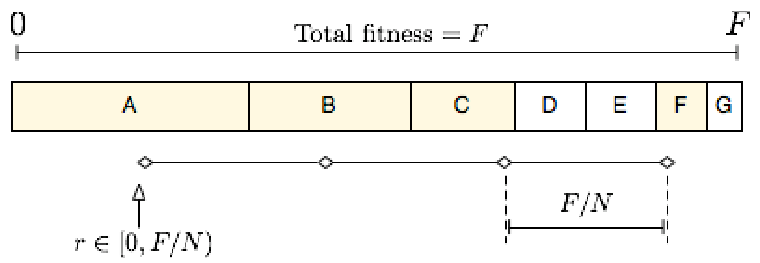
\includegraphics[width=.8\textwidth,height=0.25\textheight,keepaspectratio]
  {res/stochastic.png}
\end{figure}
\end{itemize}
\end{frame}

\begin{frame}[fragile]
\frametitle{Toán tử chọn lọc}
Để đảm bảo thế hệ sau ít nhất là tốt bằng thế hệ trước (tính theo cá thể tốt nhất của
mối thể hệ), người ta có thể đưa thêm một nhóm nhỏ các cá thể tốt nhất từ thế hệ
trước sang thế hệ sau đó. Đây được gọi là \textbf{Elitist Selection}, và nó có
thể được kết hợp với các toán tử chọn lọc trên.

Khi sử dụng \textbf{Elitist Selection}, do thế hệ sau sẽ luôn ít nhất tốt bằng
thế hệ trước, nên nếu hàm mục tiêu bị chặn, thì dãy $f_{i}$ - fitness của cá thể
tốt nhất trong thế hệ thứ $i$ là một dãy không giảm và bị chặn, do đó luôn hội
tụ đến một giá trị nào đó.

Do vậy, giải thuật di truyền luôn hội tụ đến một nghiệm tối ưu địa phương, về
mặt lý thuyết. Tuy nhiên nó có thể mất rất nhiều thế hệ để có thể thực sự tiến
gần đến điểm này.
\end{frame}

% subsection Toán tử chọn lọc (end)

\subsection{Toán tử lai ghép} % (fold)
\label{sub:Toán tử lai ghép}

\begin{frame}{One-point crossover và N-point crossover}
  \textbf{One-point crossover} (lai ghép một điểm) là một toán tử lai ghép nảy
  sinh tự nhiên như cái tên "crossover" của lai ghép.

  Khi hai nhiễm sắc thể trong thực tế thực hiện lai ghép, chúng trao đổi chéo
  với nhau (crossing over), một đoạn của nhiễm sắc thể này được chuyển sang
  nhiễm sắc thể kia và ngược lại.

\begin{figure}[t!]
    \centering
    \begin{subfigure}[t]{0.5\textwidth}
        \centering
        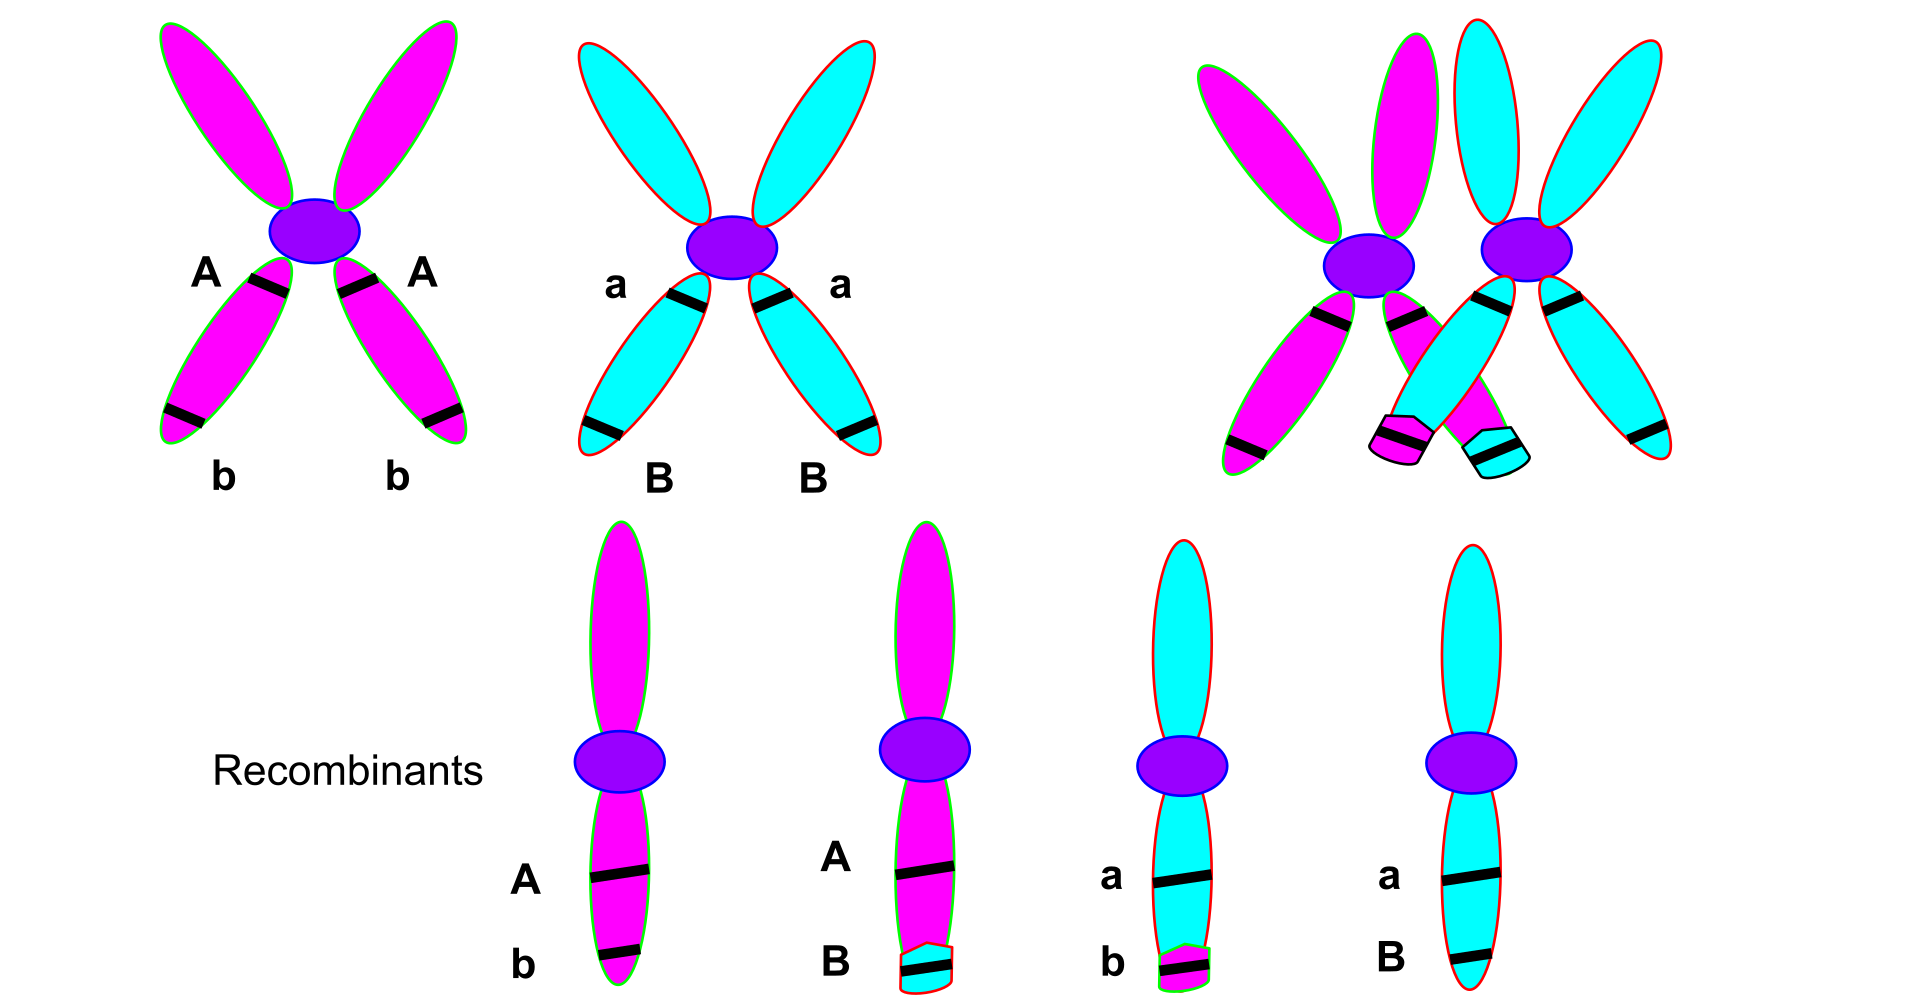
\includegraphics[height=1.2in]{res/chromosomal.png}
        \caption{Trao đổi chéo giữa hai nhiễm sắc thể}
    \end{subfigure}%
    ~ 
    \begin{subfigure}[t]{0.5\textwidth}
        \centering
        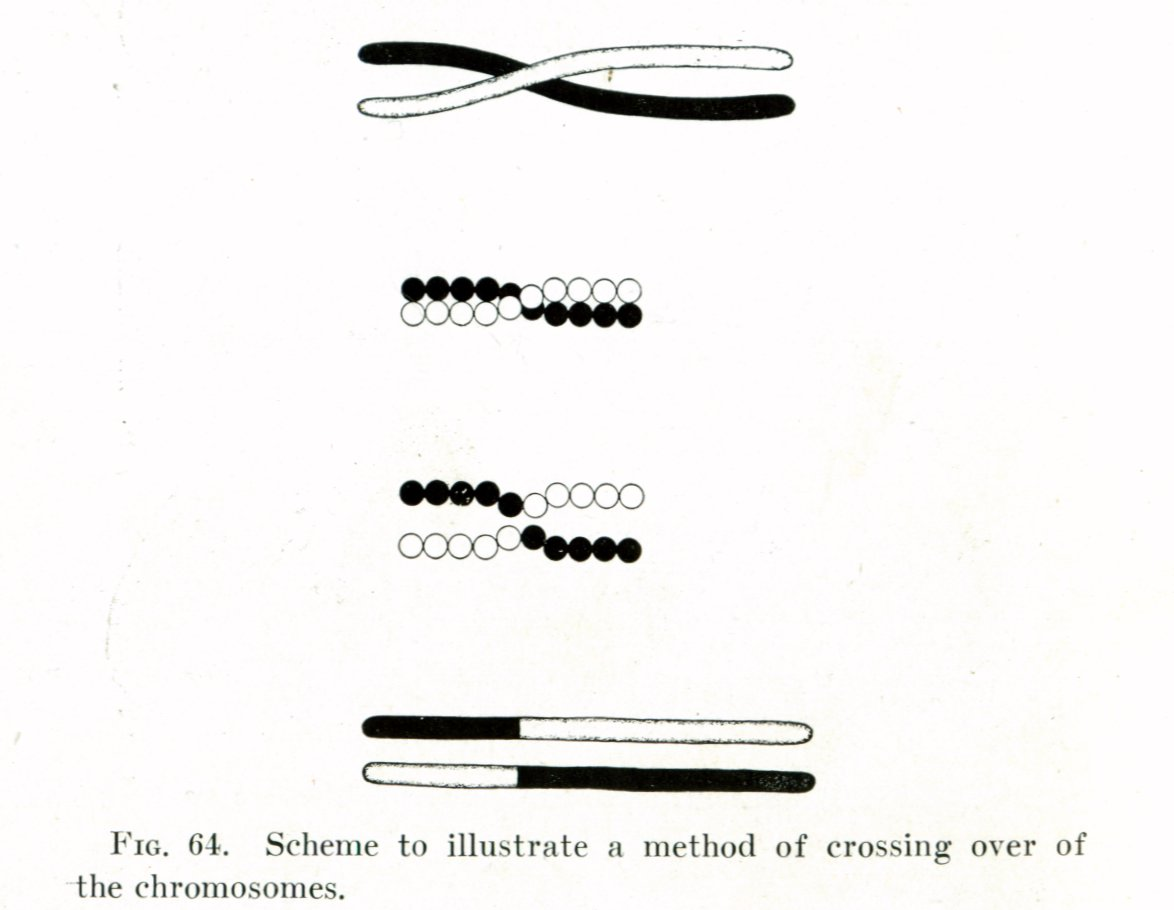
\includegraphics[height=1.2in]{res/crossover_morgan.jpg}
        \caption{Hình vẽ của T.H. Morgan về trao đổi chéo (1916)}
    \end{subfigure}
\end{figure}
\end{frame}

\begin{frame}{One-point crossover và N-point crossover}
  Ngoài one-point crossover, trao đổi chéo nhiều lần cũng xuất hiện trong tự
  nhiên, mặc dù hiếm gặp hơn. Mượn lấy ý tưởng này và tổng quát lên, ta có toán
  tử lai ghép \textbf{N-point crossover} (lai ghép $N$ điểm).

  Ý tưởng của toán tử này tương đối đơn giản: ta chọn lấy $N$ điểm cắt trên các
  nhiễm sắc thể cha mẹ, tạo ra $N + 1$ đoạn con trên mỗi nhiễm sắc thể, sau đó
  lấy xen kẽ các đoạn con để tạo ra các thể con.
\begin{figure}[t!]
    \centering
    \begin{subfigure}[t]{0.5\textwidth}
        \centering
        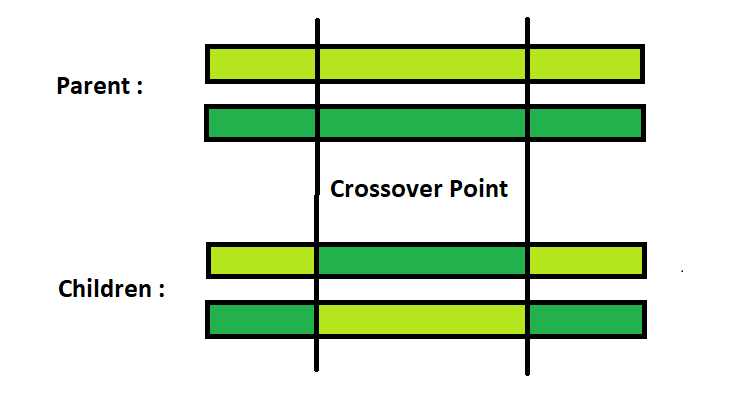
\includegraphics[height=1.2in]{res/2pco.png}
        \caption{Lai ghép hai điểm sinh ra hai cá thể con}
    \end{subfigure}%
    ~ 
    \begin{subfigure}[t]{0.5\textwidth}
        \centering
        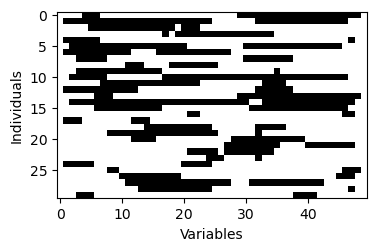
\includegraphics[height=1.2in]{res/4ptco.png}
        \caption{Các cá thể con sinh ra từ lai ghép 4 điểm}
    \end{subfigure}
\end{figure}
\end{frame}

\begin{frame}[fragile]
\frametitle{Uniform crossover}
  Một toán tử lai ghép đơn giản nữa là \textbf{Uniform crosover} (lai ghép đều).
  Mỗi gen của cá thể con sẽ được xác định bởi ngẫu nhiên, với xác suất 50\% là
  gen (cùng vị trí) của một cá thể cha mẹ và xác suất 50\% còn lại là gen cùng
  vị trí của cá thể cha mẹ còn lại.

  \begin{minted}{python}
import random

def ux(p1, p2):
  # tạo ra hai nhiễm sắc thể con là bản sao của cha mẹ
  c1 = list(p1)
  c2 = list(p2)
  for i in range(len(p1)):
    if random.random() < 0.5:
      swap(c1[i], c2[i])
  \end{minted}
\end{frame}

\begin{frame}[fragile]
\frametitle{Simulated Binary Crossover}
Vào năm 1995, Deb và Agrawal đã đề xuất ra toán tử Simulated Binary Crossover
(lai ghép nhị phân mô phỏng, SBX), mô phỏng lại toán tử One-point Crossover cho
các cá thể được mã hóa dưới dạng vector thực.

Toán tử này có các lợi thế hơn là thực hiện One-point Crossover trực tiếp trên
vector thực như giữ lại được những cấu trúc từ cá thể cha mẹ để chuyển sang đời
con, nên nó được ứng dụng rộng rãi trong giải các bài toán tối ưu phi tuyến.
\end{frame}

\begin{frame}[fragile]
\frametitle{Simulated Binary Crossover}
SBX hoạt động độc lập trên từng gen của hai nhiễm sắc thể cha mẹ. Do vậy, ta chỉ
cần xét SBX cho trường hợp số chiều bằng 1.

Giả sử hai cá thể cha mẹ (mã hóa là 2 số thực) \( p_{1}, p_{2} \) sinh ra hai cá
thể con là \( c_{1}, c_{2} \). Khi đó, theo cách làm của One-point crossover, ta
có được một bất biến:
\[
  p_{1} + p_{2} = c_{1} + c_{2}
.\] 
Như vậy, ta có thể đặc trưng một kết quả lai ghép bằng một tham số. Deb và
Agrawal sử dụng hệ số phủ (spread factor), được định nghĩa bởi:
\[
  \beta = \left| \frac{c_{1} - c_{2}}{p_{1} - p_{2}} \right| 
.\] 
\end{frame}

\begin{frame}[fragile]
\frametitle{Simulated Binary Crossover}
Từ hệ số phủ, ta dễ dàng tính lại các giá trị mã hóa của hai cá thể con:
\begin{align*}
  c_{1,2} &= \frac{1}{2}(p_{1} + p_{2}) \pm \frac{1}{2}\beta(p_{1} - p_{2})\\
  &= \frac{1}{2} \left[ (1 \pm \beta)p_{1} + (1 \mp \beta) p_{2}  \right]
.\end{align*}
Từ đây, ta có ý tưởng của SBX như sau: ta mô phỏng lai ghép nhị phân bằng cách lấy
ngẫu nhiên $\beta$ theo một phân phối nào đó, sau đó thay vào công thức để tính
ra giá trị mã hóa của các cá thể con.

Phân phối của \( \beta \) sẽ là một phân phối được lấy xấp xỉ với phân phối thực
của \( \beta \) suy ra từ thực nghiệm, và cách làm này cũng có thể được áp dụng
để mô phỏng các loại lai ghép khác.
\end{frame}

\begin{frame}[fragile]
\frametitle{Simulated Binary Crossover}
Deb và Agrawal xét giá trị \( \beta \) thu được bằng cách thực hiện One-point
Crossover với các nhiễm sắc thể mã hóa nhị phân, thu được hàm mật độ xác suất
(PDF) \( f_{\beta}(x) \) như sau:
\begin{figure}
  \centering
  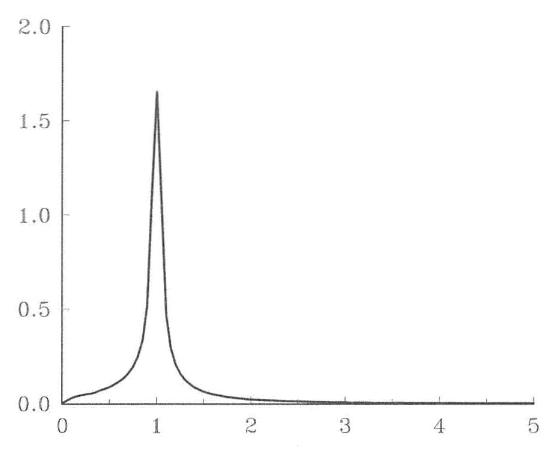
\includegraphics[height=.25\textheight]{res/sbx_pdf.png}
  \captionsetup{belowskip=0pt}
\end{figure}
Hai tác giả cho xác suất co và giãn bằng nhau, dẫn đến tính chất sau của hàm này:
\[
  f_{\beta} \left( \frac{1}{x} \right) = x^2 f_{\beta}(x), \forall x \in [0, 1]
,\] nghĩa là ta chỉ cần xác định giá trị của hàm này trên đoạn \( [0, 1] \).
\end{frame}

\begin{frame}[fragile]
\frametitle{Simulated Binary Crossover}
Do hình dạng của đồ thị hàm số \( f_{\beta} \) trên \( [0, 1] \), một lựa chọn
tự nhiên và linh hoạt để xấp xỉ hàm PDF là một hàm đa thức từng khoảng:
\[
  f_{\beta}(x) = \begin{cases}
    Cx^{\eta}, &\text{ nếu }x \in [0, 1]\\
    Cx^{-(\eta + 2)}, &\text{ nếu }x > 1
  \end{cases}
.\] 
Hệ số \( C \) dề dàng tính ra được là \( C = \frac{1}{2}(\eta  + 1) \). Số mũ \(
\eta 
\) được gọi là chỉ số của phân phối, \( \eta  \) lớn sẽ làm cho \( x \) được phân bố
dày đặc hơn ở xung quanh giá trị trung bình \( \bar{\beta} = 1 \).

Để tạo số ngẫu nhiên trong máy tính, ta sử dụng hàm ngược của hàm phân phối xác
suất (CDF), dễ dàng thu được từ hàm \( f_{\beta} \).
\[
  F^{-1}_{\beta}(\mu) = \begin{cases}
    (2\mu )^{1/(\eta  + 1)}, &\text{ nếu }\mu  < \frac{1}{2}\\
    (2(1 - \mu))^{-1/(\eta +1)}, &\text{ nếu ngược lại }
  \end{cases}
.\] 
\end{frame}

\begin{frame}[fragile]
\frametitle{Simulated Binary Crossover}
\begin{minted}[fontsize=\small]{python}
import random

eta = 3  # chỉ số phân phối
def sbx_single(p1, p2):
  mu = random.random()
  if mu < 0.5:
    beta = pow(2 * mu, 1 / (eta + 1)) 
  else:
    beta = pow(2 * (1 - mu), 1 / (eta + 1))
  return 0.5 * ((p1 + p2) + beta * (p1 - p2)),
         0.5 * ((p1 + p2) - beta * (p1 - p2))

def sbx(p1, p2):
  c1 = [0] * len(p1)
  c2 = [0] * len(p2)
  for i in range(len(p1)):
    c1[i], c2[i] = sbx_single(p1[i], p2[i])
  return c1, c2
\end{minted}
\end{frame}

\begin{frame}[fragile]
\frametitle{Order Crossover và Partially Mapped Crossover}
Các phép lai ghép trên sẽ sinh ra hai (hoặc một) cá thể con từ hai cá thể cha mẹ
với mã hóa nhiễm sắc thể dạng mảng. Tuy nhiên, nó không đảm bảo mảng nhiễm sắc
thể của cá thể con thỏa mãn những tính chất mà các cá thể cha mẹ đã có.

Với bài toán đường đi Hamilton, nhiễm sắc thể hợp lệ cần phải có các phần tử
khác nhau, hoặc nói cách khác là một hoán vị của tập số chỉ của các đỉnh đồ thị.
Do đó, để giải quyết các bài toán này, ta cần có một phép lai ghép bảo toàn tính
chất của hoán vị từ đời cha mẹ sang đời con.

Hai toán tử \textbf{Order Crossover} (OX1) và \textbf{Partially Mapped
Crossover} (PMX) là hai toán tử lai ghép cho các hoán vị, bảo đảm không sinh ra
các phần tử trùng lặp.
\end{frame}

\begin{frame}[fragile]
\frametitle{Order Crossover và Partially Mapped Crossover}
\begin{itemize}
\item 
OX1 đầu tiên chọn ra một số gen (hoặc đoạn gen) trên cá thể cha mẹ đầu tiên (\(
p_{1}\)) sẽ
được chuyển thẳng sang cá thể con. Các vị trí gen còn lại trên cá thể con được
xác định thông qua việc điền các gen còn thiếu theo thứ tự xuất hiện trên cá thể
cha mẹ còn lại \( p_{2} \).

\item
PMX chọn ra một đoạn gen trên cá thể cha mẹ đầu tiên \( p_{1} \) để chuyển thẳng
sang cá thể con. Các gen nằm trên vị trí tương ứng của cá thể cha mẹ còn lại (\(
p_{2}\)), mà không xuất hiện trên đoạn được chuyển sẽ được hoán đổi vị trí với
các gen được chuyển có vị trí trên \( p_{2} \) nằm ngoài đoạn này. Các gen còn
lại có thể được chuyển thẳng từ \( p_{2} \) mà vẫn đảm bảo tính chất của hoán
vị.
\end{itemize}
\end{frame}


\begin{frame}[fragile]
\frametitle{Order Crossover và Partially Mapped Crossover}
\begin{itemize}
\item 
OX1 đầu tiên chọn ra một số gen (hoặc đoạn gen) trên cá thể cha mẹ đầu tiên (\(
p_{1}\)) sẽ
được chuyển thẳng sang cá thể con. Các vị trí gen còn lại trên cá thể con được
xác định thông qua việc điền các gen còn thiếu theo thứ tự xuất hiện trên cá thể
cha mẹ còn lại \( p_{2} \).
\begin{align*}
  p_{1} &= (1, 2, \underline{3, 4}, 5) \\
  p_{2} &= (3, 5, 2, 4, 1)\\
  \implies c &= (?, ?, \underline{3, 4}, ?) \\
  p_{2}' &= (\cancel{3}, 5, 2, \cancel{4}, 1) \to  (5, 2, 1) \\
  \implies c&= (\underline{5, 2}, 3, 4, \underline{1})
.\end{align*}

Lượng thông tin di truyền chuyển giao từ cá thể cha mẹ sang cá thể con có thể
được cải thiện bằng cách cải tiến toán tử này thành toán tử \textbf{Order-based
Crossover} (OX2) hoặc \textbf{Position-based Crossover} (POS).
\end{itemize}
\end{frame}

\begin{frame}[fragile]
\frametitle{Order Crossover và Partially Mapped Crossover}
\begin{itemize}
\item 
PMX chọn ra một đoạn gen trên cá thể cha mẹ đầu tiên \( p_{1} \) để chuyển thẳng
sang cá thể con. Các gen nằm trên vị trí tương ứng của cá thể cha mẹ còn lại (\(
p_{2}\)), mà không xuất hiện trên đoạn được chuyển sẽ được hoán đổi vị trí với
các gen được chuyển có vị trí trên \( p_{2} \) nằm ngoài đoạn này. Các gen còn
lại có thể được chuyển thẳng từ \( p_{2} \) mà vẫn đảm bảo tính chất của hoán
vị.
\begin{align*}
  p_{1} &= (1, 2, 3, \underline{4, 5, 6}, 7, 8) \\
  p_{2} &=  (3, 7, 5, 1, 6, 8, 2, 4) \\
  \implies c &= (?, ?, ?, \underline{4, 5, 6}, ?, ?) \\
  p_{2}' &= (\cdot, \cdot, \cdot, \underline{\mathbf{1}, 6, \mathbf{8}}, \cdot,
  \cdot) \\
  p_{2}'' &= (\cdot, \cdot, 5, \cdot, \cdot, \cdot, \cdot, 4) \\
  \implies c &= (?, ?, 8, 4, 5, 6, ?, 1) \\
  \implies c&= (3, 7, 8, 4, 5, 6, 2, 1)
.\end{align*}
\end{itemize}
\end{frame}

% subsection Toán tử lai ghép (end)

\subsection{Toán tử đột biến} % (fold)
\label{sub:Toán tử đột biến}

\begin{frame}{Toán tử đột biến}
Toán tử đột biến nhằm tăng tính đa dạng cho quần thể bằng cách ngẫu nhiên làm
gây ra những thay đổi nhỏ trong cấu trúc gen của các nhiễm sắc thể.

Trong sinh học, có đột biến cấu trúc nhiễm sắc thể, nhưng do ta đang xét một cá
thể là một nhiễm sắc thể, nên cách làm này không phù hợp. Trong đột biến gen còn
có các dạng đột biến như thêm, bớt, làm thay đổi độ dài của nhiễm sắc thể, nên
cũng ít được sử dụng trong các giải thuật tiến hóa.

Vì vậy, toán tử đột biến trong các giải thuật tiến hóa thường được mô hình theo
dạng đột biến thay thế một hoặc một số gen.

\end{frame}
\begin{frame}{Toán tử đột biến}
\begin{figure}
  \centering
  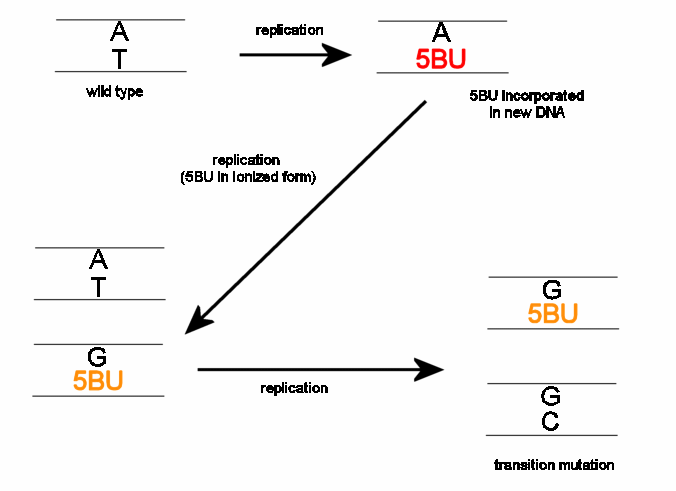
\includegraphics[width=.8\textwidth,height=0.7\textheight,keepaspectratio]
  {res/5bu.png}
  \caption{Đột biến thay thế gen xảy ra do 5BU (5-Bromouracil)}
\end{figure}
\end{frame}

\begin{frame}[fragile]
\frametitle{Bit String Mutation}
  \textbf{Bit String Mutation} là toán tử đột biến đơn giản nhất. Nó mô phỏng
  lại quá trình đột biến thay thế gen bằng cách đảo một (hoặc một số) gen
  được chọn ngâu nhiên trên nhiễm sắc thể.
  \begin{align*}
    b &= (0, 1, 0, \mathbf{0}, 1, 0) \in \{0, 1\} ^{6}\\
    \to b' &= (0, 1, 0, \mathbf{1}, 1, 0)
  .\end{align*}

  \begin{minted}{python}
import random

def bit_string_mutate(x):
  for i in range(len(x)):
    if random.random() < bit_string_mutate_rate:
      # đảo bit ngẫu nhiên
      x[i] = not(x[i])
  \end{minted}
\end{frame}

\begin{frame}[fragile]
\frametitle{Đột biến vector thực nhờ phân phối chuẩn}
Khi mở rộng Bit String Mutation cho các loại mã hóa phức tạp hơn như vector số
thực, ta sẽ gặp phải vấn đề là không biết chọn giá trị nào để thay thế cho những
gen được chọn ngẫu nhiên.

Một cách tự nhiên để giải quyết vấn đề này là tạo ra một gen ngẫu nhiên thay thế
cho mỗi gen đột biến.

Một cách thông dụng hơn là sử dụng một biến ngẫu nhiên phân phối chuẩn để cộng
thêm vào gen đột biến:
\[
  x \coloneqq  x + \Delta x,\, \Delta x \sim \mathcal{N}(0, \sigma)
.\] 

Biến ngẫu nhiên này tượng trung cho lượng nhiễu (noise) sinh ra do đột biến,
được mô phỏng qua phân phối chuẩn.
\end{frame}

\begin{frame}[fragile]
\frametitle{Đột biến vector thực nhờ phân phối chuẩn}
Nếu gen \( x \) cần nằm trong đoạn \( [a, b] \), thì độ lệch chuẩn của biến ngẫu
nhiên \( \Delta x \) có thể được tính thông qua độ dài của đoạn này:
\[
  \sigma = \frac{b - a}{6}
.\] 

Mẫu số \( 6 \) nảy sinh trong tính toán. Theo luật \( 68-95-99.7 \) trong thống
kê, thì khoảng \( 99.7\% \approx 100\% \) các giá trị trong phân phối chuẩn
cách xa giá trị trung bình nhiều nhất \( 3\sigma \). Do đó, \( [- 3\sigma, 
3\sigma] \), chứa hầu như tất cả các giá trị đáng kể của phân phối này, nên một
cách tự nhiên, ta sẽ muốn khoảng này có cùng độ dài với khoảng giá trị của \( x
\).

Sau khi cộng \( \Delta x \) vào gen \( x \), ta cần phải "kẹp" (clamp) lại biến
\( x \) này trong khoảng giá trị của nó, không cho phép nó ra ngoài \( [a, b]
\).
\end{frame}

\begin{frame}[fragile]
\frametitle{Relative Parameter Mutation}
Vì tạo số ngẫu nhiên theo phân phối chuẩn tương đối kém hiệu quả trên máy tính,
người ta đề xuất ra một cách đột biến tương tự, gọi là \textbf{Relative
Parameter Mutation} (đột biến tham số tương đối).
\begin{itemize}
\item Đầu tiên, ta xác định nên tăng hay giảm giá trị của gen này bằng một biến
  ngẫu nhiên với xác suất bằng nhau.
\item Giả sử như ta tiến hành tăng giá trị cho gen, nghĩa là giá trị mới \( x'
  \) phải nằm trong đoạn \( [x, b] \).
\item Ta xét \( k \) đoạn \( I_{i} = \left[ x, \frac{i}{k}(b - x) \right], i \in
  \{1, 2, \ldots ,k\}  \), và chọn ra một đoạn ngẫu nhiên trong những đoạn này.
  Sau đó, ta tiếp tục chọn ra một số ngẫu nhiên từ đoạn vừa chọn và lấy đây làm
  giá trị mới cho gen.
\end{itemize}

  Cách làm này, giống như cách sử dụng phân phối chuẩn cũng làm xuất hiện
  nhiều thay đổi nhỏ hơn là thay đổi lớn, do giá trị mới gần với giá trị cũ sẽ
  nằm ở trong nhiều đoạn \( I_{i} \) hơn và sẽ có xác suất được chọn cao hơn.
\end{frame}

\begin{frame}[fragile]
\frametitle{Polynomial Mutation}
Một hướng khác cải thiện cho cách đột biến dùng phân phối chuẩn là sử dụng một
phân phối khác dễ tính hơn. Chẳng hạn, \textbf{Polynomial Mutation} dựa vào phân
phối của biến \( \beta \) trong SBX để tính \( \Delta x \):
\begin{align*}
  \Delta x = \beta' \Delta x_{\text{max}}
.\end{align*}

Ở đây, \( \beta' \) nằm trong đoạn \( [-1, 1] \), khác với \( \beta \in [0,
+\infty) \), nên ta cần có điều chỉnh lại công thức tính \( \beta \) thành:
\[
  F^{-1}_{\beta'}(\mu) = \begin{cases}
    (2x)^{1 / (n+1)} - 1, &\text{ nếu }\mu < \frac{1}{2}\\
    -(2(1 - x))^{1 / (n+1)} + 1, &\text{ nếu ngược lại }
    
  \end{cases}
.\] 
\end{frame}

\begin{frame}[fragile]
\frametitle{Đột biến cho hoán vị}
Các toán tử đột biến không bảo toàn tính chất của hoán vị, nên với cách mã hóa
các nhiễm sắc thể bằng một hoán vị, cần sử dụng các toán tử đột biến đặc biệt:
\begin{itemize}
\item Đột biến Twors: đổi chỗ hai gen bất kì trên nhiễm sắc thể.
  \[
  x = (\underline{1}, 2, \underline{3}, 4) \to x' = (\underline{3}, 2,
  \underline{1}, 4)
  .\] 
\item Đột biến trượt: chọn một dãy gen con của nhiễm sắc thể, sau đó trượt
  (rotate) các gen trong dãy này.
  \[
    x = (\underline{1, 2, 3}, 4) \to x' = (\underline{3, 1, 2}, 4)
  .\] 
\item Đột biến đảo: chọn một dãy gen con của nhiễm sắc thể, sau đó đảo ngược thứ
  tự các gen trong dãy này.
  \[
    x = (\underline{1, 2, 3}, 4) \to x' = (\underline{3, 2, 1}, 4)
  .\] 
\end{itemize}
\end{frame}
% subsection Toán tử đột biến (end)

\subsection{Ứng dụng giải thuật di truyền để giải bài toán người bán hàng} % (fold)
\label{sub:Ứng dụng giải thuật di truyền để giải bài toán người bán hàng}

\begin{frame}{Ứng dụng giải thuật di truyền để giải bài toán người du lịch}
  Việc sử dụng giải thuật di truyền cho một bài toán chỉ gồm \textbf{chọn các
  toán tử di truyền phù hợp}, \textbf{khởi tạo quần thể}  và \textbf{cài đặt hàm
  fitness}.

  Trong phần này, ta xét một ví dụ cụ thể: bài toán người bán hàng (Travelling
  Salesman Problem, TSP). Cho một đồ thị \( G = (V, E) \), mỗi cạnh \( e \in E \) có
  tương ứng một độ dài \( \ell(e) \). Bài toán TSP cần tìm ra chu trình
  Hamilton (đi qua mọi đỉnh của đồ thị đúng một lần) có độ dài các cạnh là nhỏ
  nhất:
  \[
\begin{aligned}
  &&\min\, \ell(C) &= \sum_{i = 1}^{n} \ell(v_{i}v_{i+1})\\
  &&\text{subject to}\, C &= v_{1}v_{2}\ldots v_{n}v_{1},\\
  &&{} V &= \{v_{1}, v_{2}, \ldots , v_{n}\}, \\
  &&{} v_{n+1} &= v_{1}; v_{i}v_{i + 1} \in E, \forall i=\overline{1,n}\\
  && (n &= |V|)
.\end{aligned}
  \] 
\end{frame}

\begin{frame}[fragile]
\frametitle{Ứng dụng giải thuật di truyền để giải bài toán người du lịch}
  Cài đặt hàm fitness chỉ đơn thuần là tính tổng độ dài các cạnh theo công thức:
  \begin{minted}{python}
def fitness(cycle):
  return sum(length(cycle[i], cycle[i + 1])
             for i in range(-1, len(cycle) - 1))
  \end{minted}

  Khởi tạo các cá thể ngẫu nhiên cũng chỉ đơn thuần là tạo ra một hoán vị ngẫu
  nhiên của tập đỉnh. Vậy ta chỉ còn lại việc tìm các toán tử thích hợp:

  \begin{itemize}
  \item Chọn lọc: mọi cách chọn lọc đều có thể sử dụng được.
  \item Lai ghép: các cách lai ghép cho hoán vị đều có thể sử dụng được. Ta có
    thể chọn OX1 hoặc PMX.
  \item Đột biến: để đơn giản, ta có thể sử dụng đột biến Twors.
  \end{itemize}
\end{frame}
% subsection Ứng dụng giải thuật di truyền để giải bài toán người du lịch (end)


\section{Tiến hóa vi phân (Differential Evolution)} % (fold)
\label{sec:Tiến hóa vi phân (Differential Evolution)}

\subsection{Giới thiệu và thuật toán chung} % (fold)
\label{sub:Giới thiệu và thuật toán chung}

\begin{frame}{Giới thiệu chung}
  \textbf{Differential Evolution} (DE) là một giải thuật tiến hóa tương đối nổi
  tiếng sau giải thuật di truyền (GA). Được lần đầu công bố lần đầu bởi R. Storn
  và K. Price vào năm 1995, giải thuật được ứng dụng rộng rãi trong việc giải
  các bài toán tối ưu phi tuyến.

  DE được cài đặt đơn giản hơn GA, nhưng ý tưởng của nó không được tự nhiên
  bằng. Dù vậy, DE, trong nhiều trường hợp, có thể đưa ra những kết quả tốt hơn
  GA và các giải thuật di truyền khác. Tính đơn giản của DE cũng làm cho thuật
  toán này dễ dàng được ứng dụng và mở rộng. Tuy nhiên, DE chỉ có thể được áp
  dụng để giải các bài toán tối ưu liên tục.

  Thuật ngữ \textit{Differential} có thể được dịch thành \textit{vi phân}, nhưng
  thực chất thuật toán không sử dụng đạo hàm. Từ này nên hiểu theo nghĩa là sự
  chênh lệch và sai khác (giống chữ \textit{difference}) giữa các cá thể.
  Lượng chênh lệch này sẽ được sử dụng để thực hiện đột biến các cá thể trong giải
  thuật.
\end{frame}

\begin{frame}[fragile]
\frametitle{Thuật toán chung}
  DE sử dụng các toán tử lai ghép, đột biến và chọn lọc giống như GA. Tuy nhiên
  toán tử chọn lọc được định sẵn: cá thể con chỉ được thêm vào quần thể nếu nó
  tốt hơn cá thể cha mẹ của nó.
  \begin{minted}[fontsize=\footnotesize]{python}
def de():
  population = init_pop()
  while True:
    # lặp với mọi cá thể trong quần thể
    for parent in population:
      # tạo một cá thể đột biến từ các cá thể khác trong quần thể
      mutant = new_mutant(population, parent)
      # thực hiện lai ghép giữa cá thể đột biến và cá thể gốc
      offspring = crossover(parent, mutant)
      if fitness(mutant) > fitness(parent):
        # nếu cá thể con tốt hơn cá thể gốc,
        # cá thể con sẽ thay thế cá thể gốc trong quần thể
        population[population.index(parent)] = offspring
    yield population
\end{minted}
\end{frame}

% subsection Giới thiệu và thuật toán chung (end)

\subsection{Toán tử lai ghép và đột biến trong DE} % (fold)
\label{sub:Toán tử lai ghép và đột biến trong DE}

\begin{frame}{Toán tử lai ghép trong DE}
Về mặt lý thuyết, mọi toán tử lai ghép ứng dụng được cho các mảng số thực đều có
thể sử dụng được cho DE. Tuy nhiên trong thực tế, DE thường chỉ sử dụng một
trong hai loại lai ghép sau:
\begin{itemize}
\item Lai ghép nhị thức (Binomial Crossover) có thể coi là một biến dạng của Uniform
  Crossover. Mỗi gen của cá thể con sẽ được cho là gen tương ứng của cá thể gốc
  hoặc của cá thể đột biến tùy theo giá trị của một biến ngẫu nhiên:
  \[
    offspring_{i} = \begin{cases}
      mutant_{i}, &\text{ nếu } \operatorname{rand}() < CR\\
      parent_{i}, &\text{ nếu ngược lại }
      
    \end{cases}
  .\] 

  Ở đây, tham số \( CR \in [0, 1] \) (crossover rate, tỉ lệ lai ghép), ảnh hưởng
  trực tiếp đến việc chọn gen từ cá thể nào. \( CR \) càng gần \( 1 \), thì cá
  thể con càng giống như cá thể gốc.
\end{itemize}
\end{frame}

\begin{frame}{Toán tử lai ghép trong DE}
Cách làm này có thể sinh ra những cá thể con giống y hệt cá thể gốc, đặc biệt
nếu \( CR \) gần với \( 1 \). Khi đó, cá thể con chắc chắn sẽ không được lựa
chọn vào thay cho cá thể gốc, nên ta nên tránh trường hợp này xảy ra bằng cách
ép cá thể con lấy ít nhất một gen từ cá thể đột biến:
  \[
    offspring_{i} = \begin{cases}
      mutant_{i}, &\text{ nếu } \operatorname{rand}() < CR \text{ hoặc } i = R\\
      parent_{i}, &\text{ nếu ngược lại }
      
    \end{cases}
  ,\] 
  trong đó \( R \) là một chỉ số cố định cho mọi chỉ số \( i \), được chọn ngẫu
  nhiên khi bắt đầu lai ghép.
\end{frame}

\begin{frame}{Toán tử lai ghép trong DE}
\begin{itemize}
\item Toán tử lai ghép mũ (Exponential Crossover) là một toán tử có nguồn gốc từ
  Two-point Crossover. Cụ thể hơn, ta sẽ thay thế một đoạn trên cá thể gốc
  bởi đoạn tương ứng trên cá thể đột biến để thu được cá thể con.

  Điểm khác biệt giữa toán tử này với Two-point Crossover là đoạn thay thế này
  có thể "tràn" modulo, trở thành hai đoạn con ở đầu và cuối nhiễm sắc
  thể.
\end{itemize}
  \begin{figure}
    \centering
    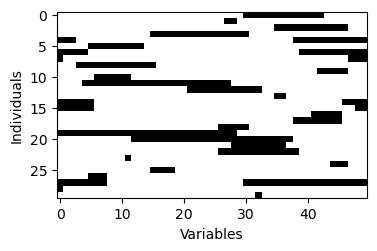
\includegraphics[height=0.5\textheight]{res/xx.png}
    \caption{Các cá thể con sinh ra từ Exponential Crossover}
  \end{figure}
\end{frame}

\begin{frame}{Toán tử đột biến trong DE}
  Toán tử đột biến chính là điểm đặc trưng lớn nhất của DE. Như cái tên của
  thuật toán, ta sẽ thực hiện đột biến bằng các giá trị chênh lệch giữa các
  vector cá thể.

  Ý tưởng chung của toán tử đột biến là ta chọn ra một cá thể cơ sở \( b \) (base) và
  một nhóm các cá thể \( G = \{g_{1}, g_{2}, \ldots , g_{|G|}\}  \). Căn cứ vào
  độ chênh lệch \( \operatorname{diff}(G) \) giữa các cá thể trong \( G \), ta
  cộng thêm một lượng vào vector \( b \) để thu được cá thể đột biến:
  \[
    mutant = b + F \cdot \operatorname{diff}(G)
  .\] 
  Để sử dụng nhiều thông tin từ quần thể, ta chọn các cá thể \( b, g_{1}, g_{2},
  \ldots , g_{|G|} \) phân biệt và khác với cá thể gốc \( parent \).

  \( F \) là một tham số được nhân vào độ chênh lệch để thu được vector được
  thêm vào cá thể cơ sở.
\end{frame}

\begin{frame}{Toán tử đột biến trong DE}
  Trong trường hợp đơn giản nhất, ta lấy nhóm \( G \) có hai phần tử: \( G =
  \{g_{1}, g_{2}\}   \). Khi đó, hàm độ chênh lệch tự nhiên nhất là hiệu của 2
  vector này:
  \begin{align*}
    \operatorname{diff}(G) &=  g_{2} - g_{1}\\ 
    \implies mutant &= b + F(g_{2} - g_{1})
  .\end{align*}
  Tham số \( F \) ở đây sẽ được chọn bằng một số thực trong đoạn \( [0, 2] \).
  \begin{figure}
    \centering
    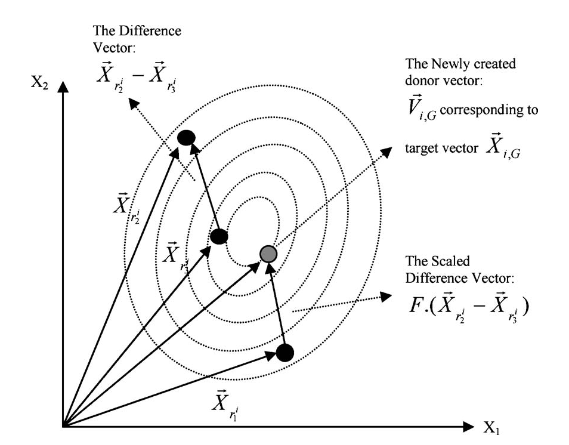
\includegraphics[height=0.4\textheight]{res/de2d.png}
    \caption{Minh họa cho phép đột biến của DE trong 2 chiều}
  \end{figure}
\end{frame}

\begin{frame}{Toán tử đột biến trong DE}
  Ta có thể thiết lập các toán tử đột biến phức tạp hơn một cách tương tự. Chẳng
  hạn, ta có thể lấy nhóm \( G = \{g_{1}, g_{2}, g_{3},
  g_{4}\}   \) là 2 cặp cá thể:
  \[
    \operatorname{diff}(G) = (g_{2} - g_{1}) + (g_{4} - g_{3})
  .\] 
  Thậm chí, ta có thể sử dụng phép nhân ma trận để có những toán tử đột biến
  linh hoạt hơn nữa:
  \begin{align*}
    \operatorname{diff}(G) &= \begin{bmatrix} g_{2} - g_{1} \\ g_{4} - g_{3}
    \end{bmatrix}\\
      \implies mutant &= b + F \cdot \operatorname{diff} (G) \\
                      &= b + \begin{bmatrix} F_{1} & F_{2} \end{bmatrix}
                      \begin{bmatrix} g_{2} - g_{1} \\ g_{4} - g_{3}
                      \end{bmatrix}  \\
                      &= b + F_{1}(g_{2} - g_{1}) + F_{2}(g_{4} - g_{3}) \\
  .\end{align*}
\end{frame}

\begin{frame}{Toán tử đột biến trong DE}
  Ngoài ra, cách chọn các cá thể \( b \) và nhóm cá thể \( G \) cũng vô cùng
  phong phú. Ta có thể dùng các toán tử chọn lọc hoặc chỉ đơn giản là chọn các
  cá thể ngẫu nhiên từ quần thể.

  Một lớp các toán tử đột biến của DE được có tên chuẩn là DE/x/y,
  trong đó:
\begin{itemize}
\item x: mô tả cách chọn cá thể cơ sở \( b \): \texttt{best} là chọn cá thể tốt
  nhất, \texttt{rand} là chọn cá thể ngẫu nhiên.
\item y: số cặp phần tử tính chênh lệch trong \( G \):
  \begin{align*}
    G &= \{g_{1}, g_{2}, \ldots , g_{2y}\}  \\
    \operatorname{diff}(G) &= \sum_{k = 1}^{y} (g_{2k} - g_{2k - 1})
  .\end{align*}
\end{itemize}
\end{frame}

\begin{frame}{Toán tử đột biến trong DE}
  Chẳng hạn, ta có các toán tử đột biến thông dụng sau:
\begin{itemize}
  \item DE/rand/1: \( mutant = b_{rand} + F(g_{2} - g_{1}) \).
\item DE/best/1: \( mutant = b_{best} + F(g_{2} - g_{1}) \).
\item DE/best/2: \( mutant = b_{best} + F(g_{2} - g_{1}) + F(g_{4} - g_{3}) \).
\item DE/target-to-best/1: \( mutant = b_{rand} + F(b_{best} - b_{rand}) +
  F(g_{2} - g_{1}) \).
\end{itemize}

Trong đó, toán tử thông dụng nhất là DE/rand/1.

\end{frame}
% subsection Toán tử lai ghép và đột biến trong DE (end)

\begin{frame}{Contour Matching}
  K. Price \textit{et al.} tìm ra một tính chất của các phép đột biến này, gọi là
  \textbf{Contour Matching}, để giải thích tính ưu việt của thuật toán DE.

  Contour Matching là hiện tượng xảy ra trong DE khi quần thể thich nghi theo
  hàm fitness dẫn đến những khu vực tiềm năng sẽ được khám phá ngay khi chúng
  được tìm ra. Các vector chênh lệch tính toán như trên thỏa mãn tính chất này,
  cả về mặt độ lớn lẫn hướng.

  Chẳng hạn, khi quần thể tiến hóa gồm hai nhóm đang tiếp cận đến hai điểm tối
  ưu địa phương, thì trong số các vector chênh lệch sẽ có hai loại: các vector gần
  bằng \( 0 \) là hiệu của 2 vector cùng nhóm, và các vector hướng từ nhóm này sang
  nhóm khác sinh ra do tính hiệu của 2 vector khác nhóm.
\end{frame}

\begin{frame}{Contour Matching}
  \begin{figure}
    \centering
    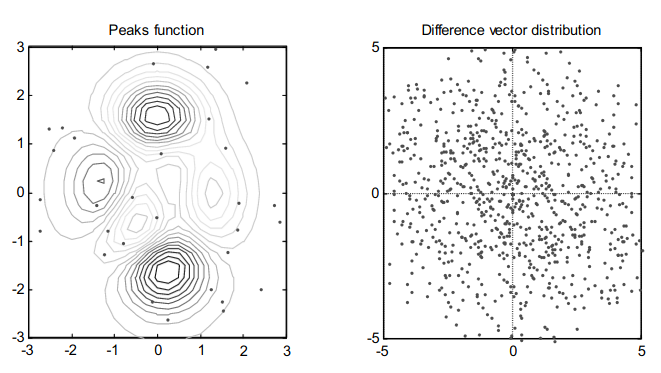
\includegraphics[width=0.8\textwidth,height=0.8\textheight,
    keepaspectratio]{res/cm1.png}
\captionsetup{justification=centering,margin=3cm}
    \caption{Ban đầu, các vector chênh lệch được phân bổ đếu ra mọi hướng.}
  \end{figure}
\end{frame}

\begin{frame}{Contour Matching}
  \begin{figure}
    \centering
    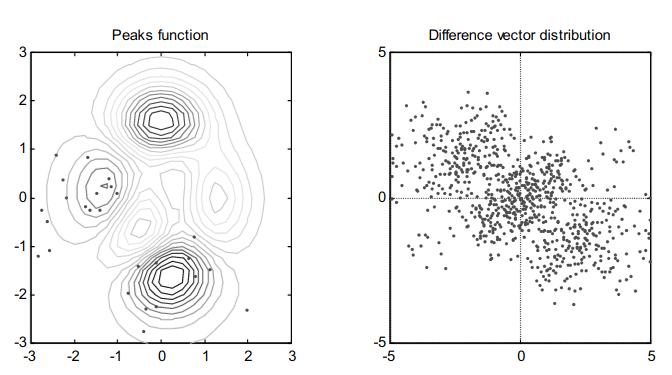
\includegraphics[width=0.8\textwidth,height=0.8\textheight,
    keepaspectratio]{res/cm2.png}
\captionsetup{justification=centering,margin=3cm}
    \caption{Khi các cá thể hội tụ đến hai nghiệm tối ưu địa phương (đỉnh), các vector
    chênh lệch bắt đầu được định hướng.}
  \end{figure}
\end{frame}

\begin{frame}{Contour Matching}
  \begin{figure}
    \centering
    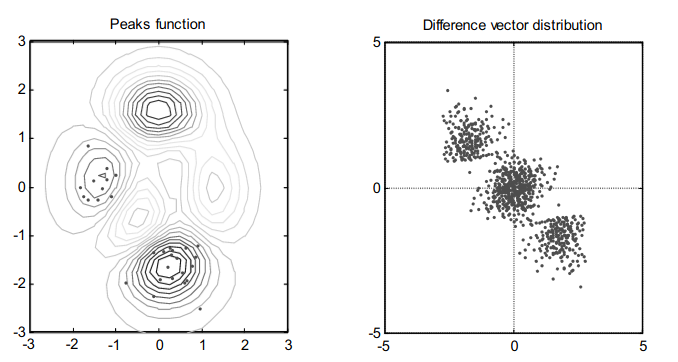
\includegraphics[width=0.8\textwidth,height=0.8\textheight,
    keepaspectratio]{res/cm3.png}
\captionsetup{justification=centering,margin=3cm}
    \caption{Các vector chênh lệch chia thành 3 nhóm: nhóm gần 0, nhóm đi từ
    một đỉnh đến đỉnh còn lại và ngược lại}
  \end{figure}
\end{frame}

\begin{frame}{Contour Matching}
  \begin{figure}
    \centering
    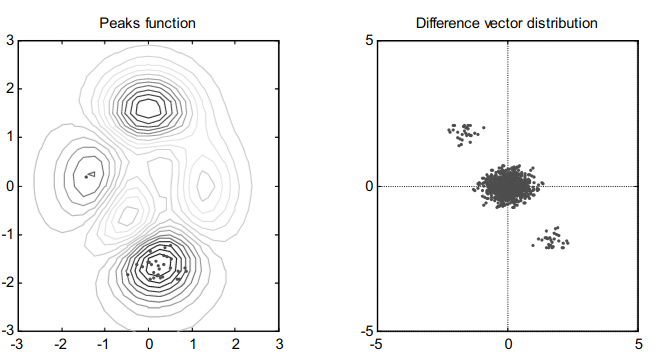
\includegraphics[width=0.8\textwidth,height=0.8\textheight,
    keepaspectratio]{res/cm4.png}
\captionsetup{justification=centering,margin=3cm}
    \caption{Sự phân bố các nhóm trở nên rõ rệt hơn. Mặt khác các cá thể hầu như
    đã hội tụ về một đỉnh, nên nhóm gần 0 đã chiếm đa số}
  \end{figure}
\end{frame}

\begin{frame}{Contour Matching}
  \begin{figure}
    \centering
    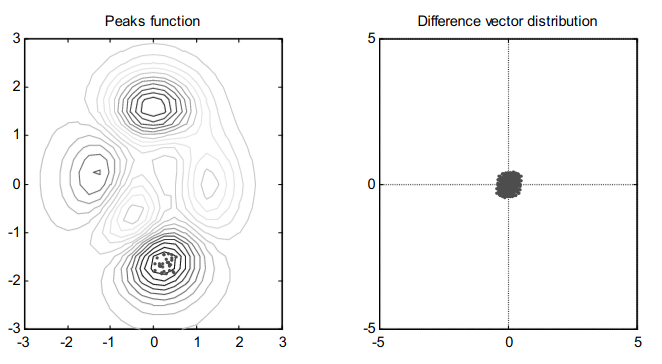
\includegraphics[width=0.8\textwidth,height=0.8\textheight,
    keepaspectratio]{res/cm5.png}
\captionsetup{justification=centering,margin=3cm}
    \caption{Các vector chênh lệch đã hội tụ về gần 0, tất cả các cá thể cũng
      hội tụ về một đỉnh}
  \end{figure}
\end{frame}

\subsection{Ảnh hưởng của các tham số đến DE} % (fold)
\label{sub:Ảnh hưởng của các tham số đến DE}

\begin{frame}{Ảnh hưởng của các tham số đến DE}
Thuật toán DE sử dụng tương đối ít tham số:
\begin{itemize}
\item \( NP \in \mathbb{N} \): số lượng cá thể trong quần thể. Tham số này được
  sử dụng để khởi tạo quần thể, và số lượng cá thể trong quần thể sẽ không đổi
  trong suốt quá trình chạy của thuật toán.
\item \( F \in [0, 2] \): gọi là trọng số vi phân (differential weight). Tham số
  này trực tiếp ảnh hưởng đến quá trình đột biến, là hệ số được nhân vào vector
  chênh lệch trước khi được thêm vào vector cơ sở.
\item \( CR \in [0, 1] \): gọi là tỉ lệ lai ghép (crossover rate). Tham số này
  càng gần 1 thì cá thể con sinh ra sau lai ghép sẽ càng giống với cá thể gốc.
\end{itemize}
\end{frame}

\begin{frame}{Ảnh hưởng của các tham số đến DE}
  \begin{itemize}
  \item 
  \textbf{Chọn} \( NP \): \( NP \) thường được chọn \( NP = 5D \) hoặc \( NP = 10D \), với \( D \) là
  số chiều của bài toán. Trong nghiên cứu của Gamperle \textit{et al.}, giá trị
  \( NP \) nằm giữa \( 3D \) và \( 8D \) sẽ cho ra kết quả tốt nhất.

  Trong thực nghiệm, một giá trị \( NP \) quá lớn cũng sẽ không làm cho thuật
  toán chạy hiệu quả hơn nhiều.

\item \textbf{Chọn} \( F \):
  Mặc dù miền giá trị của \( F \) là \( [0, 2] \), nhưng trong thực nghiệm thì
  \( F \) được chọn trong đoạn nhỏ hơn là \( [0.4, 1] \). Một giá trị hay được
  sử dụng của \( F \) là \( F = 0.5 \).

  Tuy nhiên, nếu \( F \) bàng hoặc gần \( 1 \), thì công thức đột biến nhiều khả
  năng sinh ra một cá thể đã có sẵn, làm mất đi tính đa dạng của quần
  thể. Chính vì thế, K. Price \textit{et al.} cho rằng giá trị \( F \) nên chọn
  trong khoảng \( (0.4, 0.95) \).
\end{itemize}
\end{frame}

\begin{frame}{Ảnh hưởng của các tham số đến DE}
\textbf{Chọn} \( CR \):

  Giá trị \( CR \) cần được chọn tùy thuộc vào hàm mục tiêu. Chú ý rằng khi \(
  CR = 1 \) thì vector cá thể con sẽ chỉ có 1 gen lấy tử cá thể đột biến, nên
  các toán tử đơn giản như DE/rand/1/bin sẽ có tính bất biến theo phép quay:

  \begin{itemize}
  \item Ta chọn \( CR \) là một giá trị thấp (0 hoặc 0.1) nếu như hàm fitness là
    một hàm có tính chất tương đối độc lập đối với từng gen, chẳng hạn như:
    \[
      f(x) = f_{1}(x_{1}) + f_{2}(x_{2}) + \ldots +f_{D}(x_{D})
    .\] 
  \item Nếu trường hợp ngược lại, ta cần chọn \( CR \) là một giá trị lớn hơn.
    Giá trị \( CR \) có thể được chọn trong đoạn \( [0.3, 0.9] \).
  \end{itemize}
\end{frame}

\begin{frame}{Ảnh hưởng của các tham số đến DE}
  Đã có nhiều nghiên cứu về việc cập nhật các tham số \( F \) và \( CR \) trong
  quá trình chạy thuật toán. Những thuật toán này thuộc lớp các thuật toán Adaptive
  Differential Evolution, chẳng hạn như trong SaDE (Self-adaptive Differential
  Evolution), các tham số này được cập nhật như sau:
  \begin{align*}
    F' &= \begin{cases}
      F_{l} + r_{1}(F_{u} - F_{l}), &\text{ nếu } r_{2} < \tau_{1}\\
      F, &\text{ nếu ngược lại }
    \end{cases}\\
      CR' &= \begin{cases}
      r_{3}, &\text{ nếu } r_{4}  < \tau_{2}\\
      CR, &\text{ nếu ngược lại }\\
    \end{cases}
  .\end{align*}

  Các tham số \( F_{l}, F_{u} \)\footnote{Thuật toán gốc lấy \( F_{u} \) là độ
  dài khoảng giá trị của \( F \) (\( F_{u} - F_{l} \)).} là cận dưới
  (\textbf{l}ower bound) và cận trên (\textbf{u}pper bound) của \( F \), \(
  \tau_{1} \) và \( \tau_{2} \) là các
  giá trị xác suất cho hai trường hợp, \( r_{i}, i\in \{1,2 ,3,4\}   \) là các
  số thực ngẫu nhiên giữa \( 0 \) và \( 1 \).
\end{frame}
% subsection Ảnh hưởng của các tham số đến DE (end)

% section Tiến hóa vi phân (Differential Evolution) (end)

\section{Các vấn đề chung nhất về tối ưu đa nhiệm} % (fold)
\label{sec:Các vấn đề chung nhất về tối ưu đa nhiệm}

\subsection{Tối ưu đa nhiệm} % (fold)
\label{sub:Tối ưu đa nhiệm}

\begin{frame}{Tối ưu đa nhiệm}
Ngày nay, các bài toán tối ưu xuất hiện rất nhiều trong các lĩnh vực của đời
sống như trong kỹ thuật và tổ chức. Với số lượng bài toán lớn đến như vậy, trong
đó có nhiều bài toán liên quan mật thiết với nhau, người ta nghĩ đến một cách để
kết hợp việc giải các bài toán này, sử dụng "tri thức" thu được từ giải bài toán
này để trợ giúp cho việc giải bài toán khác, làm tăng tính hiệu quả của quá
trình tối ưu.

Mô hình này được gọi là mô hình tối ưu đa nhiệm (Multitask Optimization), một
phương pháp tối ưu tương đối mới nhưng có nhiều áp dụng thực tiễn. Đặc biệt
trong bối cảnh khi mà điện toán đám mây đang phát triển, các nhà cung cấp dịch
vụ có thể sử dụng tổi ưu đa nhiệm để làm quá trình tính toán diễn ra hiệu quả
hơn.

Khác với tối ưu đa mục tiêu, tối ưu đa nhiệm tìm một nghiệm tối ưu cho mỗi bài
toán, không phải là tìm một nghiệm tối ưu cho tất cả các bài toán.
\end{frame}

\begin{frame}{Bài toán tối ưu đa nhiệm tổng quát}
  Bài toán tối ưu đa nhiệm tổng quát có dạng như sau:
\begin{align*}
  \min &\, f_{1}(x_{1}), f_{2}(x_{2}), \ldots , f_{T}(x_{T})\\
  \text{subject to}\, &x_{1} \in X_{1}, x_{2} \in X_{2},
  \ldots , x_{T} \in X_{T}.
\end{align*}

Trong đó, có \( t \) bài toán tối ưu con, thường gọi tắt là \textbf{bài toán}
(task):
\begin{alignat*}{3}
  (P_i):&&\min \, &f_i(x_i)\\
  \quad &&\text{subject to} \, &x_{i} \in X_{i}
,\end{alignat*}
với \( i \in \{1, 2, \ldots , T\}   \).

\end{frame}
% subsection Tối ưu đa nhiệm (end)
\subsection{Hai cách ngây thơ giải bài toán tối ưu đa nhiệm} % (fold)
\label{sub:Hai cách ngây thơ giải bài toán tối ưu đa nhiệm}

\begin{frame}{Hai cách ngây thơ giải bài toán tối ưu đa nhiệm}
  Một cách rất tự nhiên để giải quyết các bài toán tối ưu đa nhiệm là giải quyết
  từng bài toán con một bằng một giải thuật nào đó. Khi đó, ta có thể lựa chọn
  linh hoạt thuật toán và các tham số cho từng bài toán con, và ta cũng có thể
  dễ dàng sử dụng tính toán song song để chạy nhiều thuật toán trong cùng một
  lúc.

  Tuy nhiên, cách làm này quá độc lập, làm cho giữa các bài toán không hề có một
  lượng thông tin di truyền nào được chuyển giao. Ngoài ra, lượng tính toán và
  bộ nhớ cũng tăng tuyến tính theo số bài toán: \( O(T) \).

  Một cách khắc phục tính độc lập này là ta có thể can thiệp vào quá trình chạy
  thuật toán sau một số vòng lặp và thực hiện chuyển giao tri thức. Ý tưởng này
  được sử dụng trong một số thuật toán tối ưu đa nhiệm sẽ được đề cập trong
  những phần sau.
\end{frame}

\begin{frame}{Hai cách ngây thơ giải bài toán tối ưu đa nhiệm}
Ngoài cách xử lý riêng rẽ, ta còn có một cách ngây thơ khác để giải bài toán tối
ưu đa nhiệm. Xét bài toán tối ưu đa nhiệm tổng quát:
\begin{align*}
  \min &\, f_{1}(x_{1}), f_{2}(x_{2}), \ldots , f_{T}(x_{T})\\
  \text{subject to}\, &x_{1} \in X_{1}, x_{2} \in X_{2},
  \ldots , x_{T} \in X_{T}.
\end{align*}
Ta thấy cách biểu diễn này của một bài toán tối ưu đa nhiệm khá tương đồng với
một bài toán tối ưu đơn nhiệm. Hơn nữa, bài toán đa nhiệm trên tương đương với
bài toán đơn nhiệm sau:
\begin{align*}
  \min &\, f(x) = f_{1}(x_{1})+ f_{2}(x_{2})+ \ldots +
  f_{T}(x_{T})\\
  \text{subject to}\, &x = (x_{1}, x_{2}, \ldots, x_{T}) \in X_{1} \times  X_{2}
  \times  \ldots  \times X_{T}.
\end{align*}
Với ý tưởng này, ta có thể sử dụng các thuật toán tối ưu đơn mục tiêu như giải
thuật di truyền hay tiến hóa vi phân để giải bài toán đa nhiệm.
\end{frame}

\begin{frame}{Hai cách ngây thơ giải bài toán tối ưu đa nhiệm}
  Tuy nhiên, cách làm này lại có một số vấn đề như sau:
  \begin{itemize}
  \item Mỗi nhiễm sắc thể trong bài toán đơn nhiệm có số gen bằng tổng số chiều
    của các bài toán con, nên số chiều của bài toán này ở cỡ \( O(TD) \). Việc
    số chiều lớn sẽ làm cho các tham số của thuật toán lớn theo để giữ được khả
    năng khai phá miền nghiệm, khiến thuật toán chạy chậm hơn đáng kể.
    Vấn đề này được gọi là Curse of Dimensionality.
  \item Các bài toán con sẽ không được giải với độ ưu tiên như nhau, vì thuật
    toán sẽ có xu hướng tối thiểu hóa các bài toán dễ tối ưu trước. Ta có thể
    một phần khắc phục vấn đề này bằng cách thêm các trọng số vào hàm mục tiêu:
    \[
      f(x_{1}, x_{2}, \ldots ,x_{T}) = w_{1}f_{1}(x_{1}) + w_{2}f_{2}(x_{2}) +
      \ldots  + w_{T}f_{T}(x_{T})
    .\]
    Khi đó, cách này lại làm xuất hiện các tham số cần được điều chỉnh, làm
    phức tạp hóa việc giải bài toán này.
  \end{itemize}
\end{frame}

\begin{frame}{Hai cách ngây thơ giải bài toán tối ưu đa nhiệm}
  \begin{itemize}
  \item
    Các toán tử di truyền thông dụng trong các thuật toán như GA hay DE thường
    độc lập với từng gen, nghĩa là chỉ có các gen cùng vị trí là được kết hợp
    với nhau để sinh ra các cá thể con. Do đó, thông tin di truyền giữa các bài
    toán sẽ hầu như không được chuyển giao ra ngoài.

    Mặt khác, nếu ta cài đặt và sử dụng các toán tử di truyền cho phép chuyển
    giao thông tin di truyền giữa các bài toán với nhau, thì thông tin di truyền
    được chuyển giao mà không được điều chỉnh. Khi đó các thông tin di truyền
    tốt và xấu đều được chuyển giao với khả năng nhưa nhau.
  \end{itemize}

  Để khắc phục các vấn đề này, cần thiết kế các thuật toán chuyên dùng để giải
  các bài toán tối ưu đa nhiệm, nhằm khắc phục các vấn đề trên của cách làm ngây
  thơ.
\end{frame}

% subsection Hai cách ngây thơ giải bài toán tối ưu đa nhiệm (end)

\subsection{Sử dụng giải thuật tiến hóa trong tối ưu đa nhiệm} % (fold)
\label{sub:Sử dụng giải thuật tiến hóa trong tối ưu đa nhiệm}

\begin{frame}{Các giải thuật tiến hóa trong tối ưu đa nhiệm}
Các giải thuật tiến hóa đều có điểm chung là tiến hành cải thiện dần một quần
thể, là một nhóm các cá thể ngày càng trở nên tối ưu hơn sau các thể hệ, khác
với các giải thuật thông thường chỉ tập trung cải thiện một nghiệm duy nhất.
Điều này làm các giải thuật tiến hóa khá thích hợp cho tối ưu đa nhiệm, vì tối
ưu đa nhiệm cũng ít nhất phải thực hiện trên một nhóm các nghiệm của $T$ bài
toán.

Tiếp tục lấy ý tưởng từ tự nhiên, trong một hệ sinh thái không chỉ có một loài,
mà có rất nhiều loài sinh vật tương tác với nhau không ngừng. Hơn nữa, có một số
loài khác nhau vẫn có thể giao phối với nhau, như loài la là con lai giữa ngựa
cái và lừa đực.

Trở lại bài toán, ta sẽ coi mỗi bài toán là một loài cá thể. Giữa các loài này
có mối quan hệ tương đối gần nhau, ít nhất là các loài này có thể giao phối,
nhưng với xác suất thấp hơn là giao phối cùng loài.
\end{frame}

\begin{frame}{Các giải thuật tiến hóa trong tối ưu đa nhiệm}
  Khi áp dụng các giải thuật tiến hóa trong tối ưu đa nhiệm, việc chia loài cũng
  giúp giảm số lần tính hàm fitness. Ta sẽ chỉ tính fitness của cá thể đối với
  bài toán ứng với loài của nó, và coi fitness của nó với các bài toán còn lại
  là \( +\infty \).

  Trong thực nghiệm, các cá thể khác loại có cấu trúc gen rất khác nhau, nên ít
  khi cá thể con sinh ra lại tốt trong bài toán khác với bài toán ứng với loài
  của các cá thể cha mẹ nó. Do đó, cách giảm số lần tính fitness này không làm
  mất đi quá nhiều cá thể tiềm năng.
\end{frame}

\begin{frame}{Mã hóa trong tối ưu đa nhiệm tiến hóa}
  Cũng giống như trong tự nhiên, ta sẽ sử dụng một dạng nhiễm sắc thể cho mọi
  loài trong giải thuật. Điều này giúp cho việc cài đặt các toán tử di truyền
  không có gì khác so với các giải thuật di truyền thông thường, vì chúng vẫn
  hoạt động trên các mảng gen.

  Để thuận lợi cho các toán tử di truyền, ta sẽ cố định số gen trong mọi cá thể.
  Để sử dụng ít chiều nhất, ta sẽ chọn số chiều bằng với số chiều lớn nhất của
  các bài toán:
  \[
    D = \max\limits_{1 \le i \le T} D_{i}
  .\] 
  Cụ thể cách mã hóa như thế nào sẽ được chọn theo các bài toán con. Chẳng hạn,
  nếu các bài toán con là các bài toán rời rạc, ta có thể sử dụng các cách mã
  hóa rởi rạc như mảng hoán vị hay chuỗi nhị phân.
\end{frame}

\begin{frame}{Xử lý ràng buộc của các bài toán con}
  Cách mã hóa thống nhất của các thuật toán tối ưu đa nhiệm dẫn đến vấn đề về
  ràng buộc. Chẳng hạn như nếu ta sử dụng mã hóa mảng số thực, các ràng buộc của
  các bài toán có thể mâu thuẫn với nhau, dẫn đến việc không có một cá thể nào
  là hợp lệ.

  Để xử lý vấn đề này, ta có hai cách như sau:

  \begin{itemize}
  \item Sử dụng hàm phạt: Đối với các cá thể không hợp lệ, thay vì loại bỏ chúng
    thì ta giữ lại, nhưng cho chúng giá trị hàm fitness lớn bằng cách cộng thêm
    một hàm phạt vào hàm fitness của từng bài toán:
    \[
      f^{*}_{i}(x) = f_{i}(x) + C_{i}P_{i}(x)
    .\] 
    \( C_{i} \) là một hằng số lớn để hạn chế việc vi phạm ràng buộc.
  \end{itemize}
\end{frame}

\begin{frame}{Xử lý ràng buộc của các bài toán con}
  \begin{itemize}
  \item Thay đổi cách mã hóa: Ta thay đổi cách mã hóa của từng bài toán để loại
    bỏ đi các cá thể không thỏa mãn ràng buộc trong khi vẫn giữ nguyên dạng mã
    hóa chung. Chẳng hạn như nếu dạng mã hóa chung là \( [0, 1]^{D} \) nhưng một
    bài toán có ràng buộc \( a_{i} \le x_{i} \le b_{i}, \forall i=
    \overline{1,d} \) (\( d \le D\) là số chiều của bài toán con), ta có thể
    thực hiện nội suy tuyến tính để chuyển tử \( [0, 1]^{D} \) sang miền nghiệm:
    \[
      x' = a + x_{1..d} \odot (b - a) = 
      \begin{bmatrix} 
        a_{1} + x_{1}(b_{1}-a_{1})\\
        a_{2} + x_{2}(b_{2}-a_{2})\\
        \vdots \\
        a_{d} + x_{d}(b_{d} - a_{d})
      \end{bmatrix} 
    .\]

    Cách này khó dùng hơn so với cách sử dụng hàm phạt nhưng nó luôn cho ra kết
    quả tốt hơn do nó không phải giữ lấy các giá trị vi phạm ràng buộc.
  \end{itemize}
\end{frame}

% subsection Sử dụng giải thuật tiến hóa trong tối ưu đa nhiệm (end)

% section Các vấn đề chung nhất về tối ưu đa nhiệm (end)

\section{Thuật toán Tiến hóa Đa yếu tố (MFEA)} % (fold)
\label{sec:Thuật toán Tiến hóa Đa yếu tố (MFEA)}

\subsection{Việc phân loài trong MFEA} % (fold)
\label{sub:Việc phân loài trong MFEA}

\begin{frame}{Việc phân loài trong MFEA}
  Lấy ý tưởng từ các loài trong tự nhiên, thuật toán MFEA chia quần thể hiện tại
  thành các loài ứng với các bài toán. Một cách tự nhiên, ta có thể coi một cá thể \( p
  \) là cá thể loài \( i \) (\( i \in \{1, 2, \ldots , T\}   \)) nếu nó "phù hợp
  nhất" đối với bài toán \( i \).

  Ta cần chỉ rõ rằng một cá thể như thế nào là "phù hợp nhất"
  với một bài toán. Chẳng hạn, ta có thể sử dụng trực tiếp hàm fitness:
  \[
    i = \operatorname*{argmin}_{1 \le j \le  T} \{f_{j}(x)\}  \iff x \text{ "phù
    hợp nhất" với bài toán thứ } i
  .\] 
  Tuy nhiên, việc so sánh trực tiếp các hàm fitness không nên được dùng, do các
  hàm fitness của các bài toán khác nhau có các miền giá trị khác nhau. Do đó,
  ta sử dụng một giá trị có miền giá trị cố định hơn: thứ tự của cá thể trong
  quần thể khi sắp xếp theo thứ tự giảm dần của hàm fitness của bài toán thứ \(
  i\), hay \textbf{factorial rank} của cá thể đối với bài toán thứ \( i \):
  \[
    i = \operatorname*{argmin}_{1 \le j \le  T} \{r_{j}(x)\}  \iff x \text{ "phù
    hợp nhất" với bài toán thứ } i
  .\] 
\end{frame}

\begin{frame}{Việc phân loài trong MFEA}
  Khi xác định factorial rank, các cá thể có cùng giá trị fitness đối với bài
  toán thứ \( j \), gọi là \textbf{\( j \)-counterparts}, sẽ được sắp xếp ngẫu nhiên và
  có factorial rank khác nhau. Nếu các \( j \)-counterparts là cùng loài, chúng
  được gọi là \textbf{strong counterparts}.

  "Loài" trong MFEA được mô phỏng bởi \textbf{skill factor}. Skill factor của cá
  thể \( x \) được ký hiệu là \( \tau (x) \):
  \begin{align*}
    \tau (x) = i &\iff x \text{ "phù hợp nhất" với bài toán thứ } i\\
                 &\iff i = \operatorname*{argmin}_{1 \le j \le  T} \{r_{j}(x)\} 
  .\end{align*}

  Khi MFEA sử dụng thêm hàm phạt để hạn chế các cá thể vi phạm ràng buộc, giá
  trị của hàm fitness sau khi cộng thêm hàm phạt của một cá thể được gọi là
  \textbf{factorial cost}. Ở đây, ta coi như việc cộng thêm hàm phạt thuộc về
  từng bài toán, nên factorial cost và fitness coi như là một.
\end{frame}

\begin{frame}{Việc phân loài trong MFEA}
  Trong MFEA, mỗi cá thể có \( T \) giá trị fitness ứng với \( T \) bài toán. Để
  so sánh giữa các cá thể khác loài trong MFEA, người ta đưa ra một giá trị
  fitness chung mọi bài toán, gọi là \textbf{scalar fitness}:
  \[
    \varphi(x) = \frac{1}{\min\limits_{1 \le j \le  T} r_{j}(x)}=
    \frac{1}{r_{\tau (x)}(x)}
  .\] 
  Sử dụng scalar fitness ta có thể so sánh giữa các cá thể. Cá thể \( x \) gọi
  là \textbf{trội hơn} cá thể \( y \) nếu như nó có scalar fitness lớn hơn: \( x
  \gg y \iff \varphi(x) > \varphi(y) \).
\end{frame}

\begin{frame}{Việc phân loài trong MFEA}
  \[
    \begin{array}{c| c c c c}
      
    \end{array}
  .\] 
\end{frame}
% subsection Việc phân loài trong MFEA (end)

\subsection{Thuật toán chung của MFEA} % (fold)
\label{sub:Thuật toán chung của MFEA}

\begin{frame}[fragile]
\frametitle{Thuật toán chung của MFEA}
Về cấu trúc chung, thuật toán MFEA có dạng giống như một thuật toán tiến hóa cơ
bản. Điểm khác biệt lớn nhất là sau khi sinh ra các cá thể mới, các giá trị
skill factor và scalar fitness của mọi cá thể cần được cập nhật (hàm
$\texttt{update\_mfea\_values}$):
\begin{minted}[fontsize=\small]{python}
def mfea():
  population = init_pop()
  update_mfea_values(population)

  while True:
    reproduction(population)
    update_mfea_values(population)
    selection(population)
    yield population
\end{minted}
\end{frame}

\begin{frame}[fragile]
\frametitle{Thuật toán chung của MFEA}
Do skill factor và scalar fitness phụ thuộc vào factorial rank, nên các giá trị
này phụ thuộc vào cả quần thể chứ không phải chỉ một mình cá thể. Do đó, khi cập
nhật các giá trị này, ta cần tiến hành cập nhật với mọi cá thể trong quần thể:
\begin{minted}[fontsize=\footnotesize]{python}
def update_mfea_values(population):
  # Tính factorial rank
  for task in tasks:
    # Sắp xếp quần thể theo factorial cost (fitness)
    population.sort(key=lambda x: x.factorial_cost[task], reverse=True)
    for i, x in enumerate(population): # lặp cùng chỉ số
      x.factorial_rank[task] = i + 1 # cộng 1 do chỉ số bắt đầu từ số 0

  # Từ factorial rank tính skill factor và scalar fitness
  for x in population:
    # skill factor là bài toán mà x có factorial rank thấp nhất
    x.skill_factor = min(tasks, lambda task: x.factorial_rank[task])
    # scalar fitness tính thông qua skill factor
    x.scalar_fitness = 1 / x.factorial_rank[x.skill_factor]
\end{minted}
\end{frame}

\begin{frame}[fragile]
\frametitle{Thuật toán chung của MFEA}
\begin{minted}[fontsize=\small]{python}
def mfea():
  population = init_pop()
  update_mfea_values(population)

  while True:
    reproduction(population)
    update_mfea_values(population)
    selection(population)
    yield population
\end{minted}

Sử dụng scalar fitness, ta có thể tiến hành chọn lọc trong MFEA sử dụng các toán
tử chọn lọc như trong giải thuật di truyền. Đây cũng là lý do vì sao ta thực
hiện bước chọn lọc sau khi tính toán hết các scalar fitness và skill factor.
\end{frame}

% subsection Thuật toán chung của MFEA (end)

\subsection{Toán tử sinh sản trong MFEA} % (fold)
\label{sub:Toán tử sinh sản trong MFEA}

\begin{frame}[fragile]
\frametitle{Toán tử sinh sản trong MFEA}
MFEA lấy ý tưởng từ hai hiện tượng xảy ra trong tự nhiên và xã hội:
\begin{itemize}
\item Giao phối chọn lọc (Assortative Mating): các cá thể trong tự nhiên có xu
  hướng giao phối với các cá thể có các đặc điểm giống cá thể này. Ở đây, các cá
  thể sẽ ưu tiên giao phối cùng loài:
\begin{minted}[fontsize=\small]{python}
import random

def reproduction(population):
  for p1, p2 in pick_mating_parents(population):
    # nếu không cùng loài, chỉ thực hiện giao phối với xác suất `rmp`
    if p1.skill_factor == p2.skill_factor or random.random() < rmp:
      create_offspring(population, p1, p2) # tạo con và thêm vào quần thể
    else:
      create_mutant(population, p1) # tạo con là các đột biến của
      create_mutant(population, p2) # hai cá thể cha mẹ
\end{minted}
Ở đây, tham số $\texttt{rmp}$ (random mating probability) điều chỉnh xác suất
lai ghép khác loài.
\end{itemize}
\end{frame}

\begin{frame}[fragile]
\frametitle{Toán tử sinh sản trong MFEA}
MFEA lấy ý tưởng từ hai hiện tượng xảy ra trong tự nhiên và xã hội:
\begin{itemize}
\item Chuyển giao văn hoá dọc (Vertical Cultural Tranmission): Chuyển giao văn
  hóa có hai loại: ngang (từ các cá thể cùng thế hệ) và dọc (từ các cá thể cha
  mẹ, tổ tiên). MFEA chỉ sử dụng chuyển giao văn hóa dọc.
\end{itemize}
  \begin{figure}
    \centering
    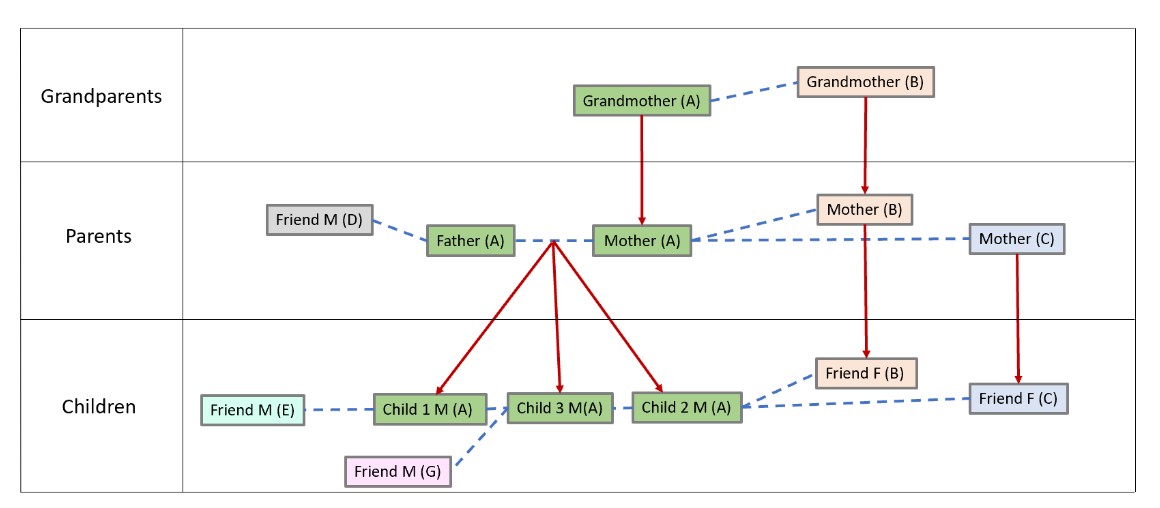
\includegraphics[height=0.5\textheight]{res/vct.png}
    \caption{Mạng các mối quan hệ của một người trong một nhóm nhỏ.}
  \end{figure}
\end{frame}

\begin{frame}[fragile]
\frametitle{Toán tử sinh sản trong MFEA}
Trong MFEA, văn hóa được chuyển giao chính là thông tin về loài. Cá thể con sẽ
kế thừa skill factor từ cá thể cha mẹ của nó:
\begin{minted}[fontsize=\footnotesize]{python}
def create_offspring(population, p1, p2):
  for c in crossover(p1, p2): # thực hiện lai ghép (có thể sinh ra nhiều con)
    # ép cá thể con phải có skill factor của một trong hai cá thể cha mẹ
    c.skill_factor = random.choice([p1.skill_factor, p2.skill_factor])
    c.factorial_cost[c.skill_factor] = fitness(c.skill_factor, c)
    population += [c]

def create_mutant(population, p): # thực hiện đột biến, tương tự như trên
  c = mutate(p)
  c.skill_factor = p.skill_factor
  c.factorial_cost[c.skill_factor] = fitness(c.skill_factor, c)
  population += [c]
\end{minted}

Khi skill factor của cá thể con được cập nhật, thì do các factorial cost của nó
đối với các bài toán khác bài toán skill factor bằng \( +\infty \), nên skill
factor của nó không đổi.
\end{frame}

% subsection Toán tử sinh sản trong MFEA (end)

\subsection{Tổng quát hóa thuật toán MFEA} % (fold)
\label{sub:Tổng quát hóa thuật toán MFEA}

\begin{frame}{Decision Variable Translation Strategy}
  Xét bài toán tối ưu đa nhiệm sau:
  \begin{align*}
    f_{1}(x) &= (x_{1}-1)^2+(x_{2}-2)^2 \\
    f_{2}(x) &=  (x_{1}+1)^2+(x_{2}+2)^2 \\
    X_{1} &= X_{2} = \mathbb{R}^2
  .\end{align*}
  Thì khi thuật toán hội tụ, các cá thể hai loài sẽ nằm lần lượt trong hai lân cận \(
  [1-\varepsilon,1+\varepsilon] \times [2-\varepsilon, 2+\varepsilon] \) và \(
  [-1-\varepsilon, -1+\varepsilon] \times [-2-\varepsilon, -2+\varepsilon] \).
  Nếu ta sử dụng các phép lai ghép như N-point Crossover hay SBX, một cá thể
  được lai từ hai loài sẽ luôn kém tối ưu hơn cha mẹ nó, nên việc chuyển giao
  tri thức không còn hiệu quả.

  Mặt khác, ta dễ thấy rằng hai hàm mục tiêu có biểu hiện trên giống y hệt nhau
  ở gần điểm cực tiểu \( (1, 2) \) và \( (-1, -2) \), nên rõ ràng vẫn có thông
  tin có thể chuyển giao giữa hai bài toán.
\end{frame}

\begin{frame}[fragile]
\frametitle{Decision Variable Translation Strategy}
  Để khắc phục vấn đề này, trước khi lai ghép, ta có thể thực hiện một bước
  \textbf{tịnh tiến} các cá thể cha mẹ lại gần nhau, sau đó thực hiện lai ghép
  và tịnh tiến ngược lại cá thể con tùy theo skill factor của cá thể này:
% https://q.uiver.app/#q=WzAsOCxbMCwwLCJwXzEiXSxbMCwyLCJwXzIiXSxbMiwwLCJwXzEnIl0sWzIsMiwicF8yJyJdLFs0LDAsImNfMSciXSxbNCwyLCJjJ18yIl0sWzYsMCwiY18xIl0sWzYsMiwiY18yIl0sWzAsMiwiVF8xIl0sWzEsMywiVF8yIiwyXSxbMyw0XSxbMiw1XSxbMiw0LCJcXHRleHR7bWF0aW5nfSJdLFszLDUsIlxcdGV4dHttYXRpbmd9IiwyXSxbNCw2LCJUXzFeey0xfSJdLFs1LDcsIlRfMl57LTF9IiwyXV0=
\[\begin{tikzcd}[cramped]
	{p_1} && {p_1'} && {c_1'} && {c_1} \\
	\\
	{p_2} && {p_2'} && {c'_2} && {c_2}
	\arrow["{T_1}", from=1-1, to=1-3]
	\arrow["{T_2}"', from=3-1, to=3-3]
	\arrow[from=3-3, to=1-5]
	\arrow[from=1-3, to=3-5]
	\arrow["{\text{mating}}", from=1-3, to=1-5]
	\arrow["{\text{mating}}"', from=3-3, to=3-5]
	\arrow["{T_1^{-1}}", from=1-5, to=1-7]
	\arrow["{T_2^{-1}}"', from=3-5, to=3-7]
\end{tikzcd}\]

Ở ví dụ trên, các cá thể cha mẹ được tịnh tiến trước khi thực hiện lai ghép,
sinh ra hai con có hai skill factor khác nhau. Hai cá thể con này sẽ được tịnh
tiến ngược lại để được thêm vào quần thể.
\end{frame}

\begin{frame}[fragile]
\frametitle{Decision Variable Translation Strategy}
Để xác định các phép tịnh tiến \( T_{i} \) cho bài toán thứ \( i \), một sự lựa
chọn tự nhiên là phép tịnh tiến thỏa mãn điều kiện sau:
\[
  T_{i}(m_{i}) = cp \implies T_{i}(x) = x + (cp - m_{i})
.\]
Trong đó, điểm \( cp \) (chẳng hạn \( cp = (0.5, 0.5, \ldots , 0.5) \)) là một
vị trí cố định trong không gian chung. \( m_{i} \) là một vector đại diện cho
các vector có loài thứ \( i \) (skill factor bằng \( i \)).

Ta có thể lấy \( m_{i} \) là vector trung bình của top \( \mu \% \) các cá thể
có loài thứ \( i \):
\begin{gather*}
  m_{i} =  \frac{1}{\mu N_{i}}\sum_{\substack{x \in P\\\tau (x) = i\\ r_{i}(x)
  \le \mu N_{i}}}(x), i=\overline{1,T}
\end{gather*}
\( N_{i} \) ở đây là số cá thể có skill factor là \( i \) trong quần thể.
\end{frame}

\begin{frame}[fragile]
\frametitle{Decision Variable Translation Strategy}
Vector tịnh tiến còn được nhân thêm với hai tham số để tối ưu việc tịnh tiến:
\begin{itemize}
\item \( sf \) (scale factor): Khi các cá thể đang hội tụ đến một điểm, vector
  \( m_{i} \) có thể chưa phản ánh đúng vị trí cực tiểu thực sự, nên vector \(
  cp-m_{i} \) có thể có sự sai lệch nhỏ. \( sf \) được nhân thêm nhằm chỉnh lại
  sai số này.

\item \( \alpha \): Do \( m_{i} \) càng ngày càng tiến đến chính xác hơn vị trí
  tối ưu, nên ta sẽ cho tham số này tăng dần trong quá trình chạy thuật toán như
  sau:
  \[
    \alpha = \left( \frac{g}{G} \right) ^2
  .\]

  Trong đó, \( g \) và \( G \) lần lượt là số thế hệ hiện tại và số thế hệ tối
  đa.
\end{itemize}
\[
  T_{i}(x) = x + sf \cdot \alpha(cp - m_{i})
.\] 
\end{frame}

\begin{frame}[fragile]
\frametitle{Decision Variable Translation Strategy}
Ngoài ra, việc liên tục cập nhật các phép tịnh tiến này sẽ làm cho thuật toán
chạy không ổn định và không thể hội tụ. Vì thế nên ta sẽ chỉ cập nhật các \(
T_{i} \) khoảng \( \theta \) thế hệ một lần.

Mặt khác, do các giá trị \( m_{i} \) không phản ánh chính xác vị trí tối ưu trong
những thế hệ đầu, nên ta sẽ chỉ bắt đầu cập nhật các \( T_{i} \) sau \( \phi \)
thế hệ.

\begin{minted}{python}
def try_update_translations(generation):
  if generation > phi and generation % theta == 0:
    update_translations(generation)
\end{minted}

Cách thực hiện tịnh tiến và cập nhật vector tịnh tiến trên được gọi là
\textbf{Decision Variable Translation Strategy} (DVTS).
\end{frame}

\begin{frame}[fragile]
\frametitle{Decision Variable Shuffling Strategy}
Tiếp tục xét bài toán sau:
\begin{align*}
  f_{1}(x) &= x_{1}^2+x_{2}^2 \\
  f_{2}(x) &= \operatorname{Ackley}(x) \\
  X_{1} &= \mathbb{R}^2, X_{2} = \mathbb{R}^{100}
.\end{align*}
Hàm \( f_{2} \) là hàm Ackley 100 chiều, một hàm số hay được sử dụng trong thử
nghiệm các thuật toán tối ưu. Hàm này có nhiều nghiệm tối ưu địa phương nên
tương đối khó tối ưu.
\begin{figure}
  \centering
  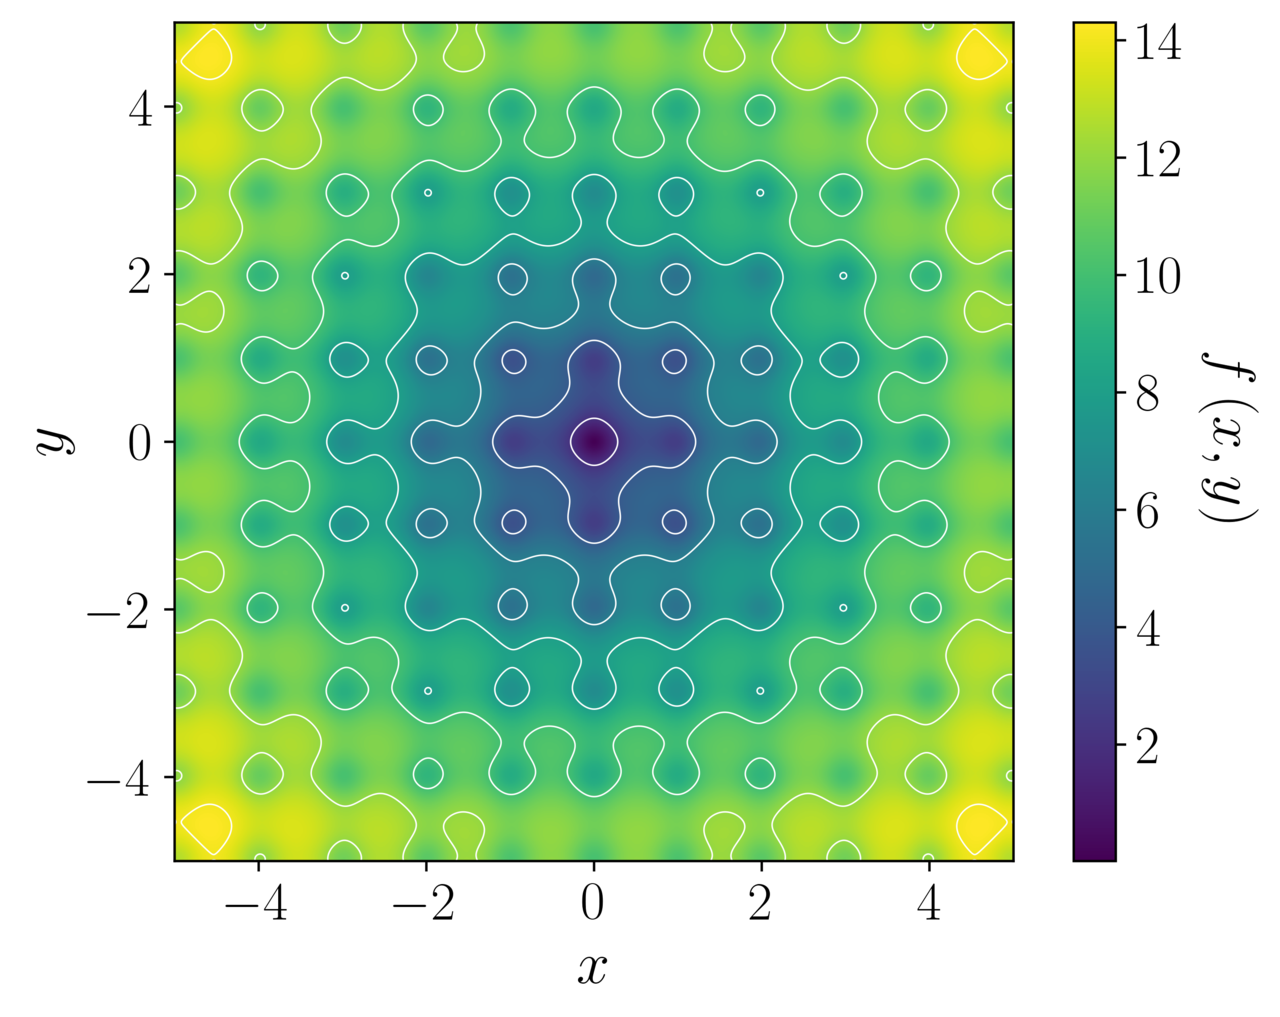
\includegraphics[height=0.3\textheight]{res/ackley.png}
  \caption{Đồ thị màu hàm Ackley trong hai chiều.}
\end{figure}
\end{frame}

\begin{frame}[fragile]
\frametitle{Decision Variable Shuffling Strategy}
\begin{align*}
  f_{1}(x) &= x_{1}^2+x_{2}^2 \\
  f_{2}(x) &= \operatorname{Ackley}(x) \\
  X_{1} &= \mathbb{R}^2, X_{2} = \mathbb{R}^{100}
.\end{align*}
Hai hàm số có cực tiểu giống nhau (đều là vector không), nên ta sẽ mong muốn
MFEA sử dụng tính tương đồng này để chuyển giao tri thức từ hàm dễ tối ưu hơn
(hàm \( f_{1} \)) sang hàm khó tối ưu hơn (hàm \( f_{2} \)).

Tuy nhiên, thuật toán hiện tại của ta chỉ có thể chuyển giao được tri thức của
hai gen đầu, vì số chiều của bài toán thứ nhất chỉ bằng 2. Nếu lựa chọn phép đột
biến phù hợp, thì thông tin di truyền từ hai gen đầu này cũng có thể được chuyển
sang các gen khác do toán tử đột biến, nhưng nhìn chung, ta sẽ muốn quá trình
chuyển giao tri thức trực tiếp làm điều này.
\end{frame}

\begin{frame}[fragile]
\frametitle{Decision Variable Shuffling Strategy}
Ta có thể sử dụng ý tưởng trước của phép tịnh tiến, thay phép tịnh tiến bằng
một phép hoán vị:
% https://q.uiver.app/#q=WzAsOCxbMCwwLCJwXzEiXSxbMCwyLCJwXzIiXSxbMiwwLCJwXzEnIl0sWzIsMiwicF8yJyJdLFs0LDAsImNfMSciXSxbNCwyLCJjJ18yIl0sWzYsMCwiY18xIl0sWzYsMiwiY18yIl0sWzAsMiwiXFxzaWdtYV8xIl0sWzEsMywiXFxzaWdtYV8yIiwyXSxbMyw0XSxbMiw1XSxbMiw0LCJcXHRleHR7bWF0aW5nfSJdLFszLDUsIlxcdGV4dHttYXRpbmd9IiwyXSxbNCw2LCJcXHNpZ21hXzFeey0xfSJdLFs1LDcsIlxcc2lnbWFfMl57LTF9IiwyXV0=
\[\begin{tikzcd}[cramped]
	{p_1} && {p_1'} && {c_1'} && {c_1} \\
	\\
	{p_2} && {p_2'} && {c'_2} && {c_2}
	\arrow["{\sigma_1}", from=1-1, to=1-3]
	\arrow["{\sigma_2}"', from=3-1, to=3-3]
	\arrow[from=3-3, to=1-5]
	\arrow[from=1-3, to=3-5]
	\arrow["{\text{mating}}", from=1-3, to=1-5]
	\arrow["{\text{mating}}"', from=3-3, to=3-5]
	\arrow["{\sigma_1^{-1}}", from=1-5, to=1-7]
	\arrow["{\sigma_2^{-1}}"', from=3-5, to=3-7]
\end{tikzcd}\]
Ở đây, phép hoán vị sẽ làm thay đổi vị trí các gen trên nhiễm sắc thể trước khi
thực hiện lai ghép. Khi đó, dễ thấy các gen 1, 2 của bài toán trên sẽ có thể
được chuyển sang các vị trí mới, thực hiện chuyển giao tri thức sang các gen ở vị
trí này.
\end{frame}

\begin{frame}[fragile]
\frametitle{Decision Variable Shuffling Strategy}
Giả sử ta đang thực hiện lai ghép giữa hai cá thể khác loài \( x \) và \( y \),
tương ứng với hai bài toán 1 và 2 có số chiều lần lượt là \( D_{1} \) và \(
D_{2} \).

Nếu \( D_{1} = D_{2} \), ta có thể thực hiện lai ghép mà không cần hoán vị.

Nếu \( D_{1} < D_{2} \), không mất tính tổng quát, giả sử \( D_{1} < D_{2} \).
Chỉ \( D_{1} \) gen đầu của \( x \) chứa tri thức từ bài toán 1, còn \( D_{2} -
D_{1}\) gen còn lại có thể coi như là ngẫu nhiên. Do đó, thay vì sử dụng những
gen ngẫu nhiên này, ta có thể thay thế các gen này bởi các gen của một cá thể \(
y^{*} \) khác có cùng skill factor với \( y \):
\[
  x'_{\sigma_{1}(i)} = \begin{cases}
    x_{i}, &\text{ nếu } 1 \le i \le D_{1}\\
    y^{*}_{\sigma_{1}(i)}, &\text{ nếu ngược lại }\\
  \end{cases}
.\] 
\end{frame}

\begin{frame}[fragile]
\frametitle{Decision Variable Shuffling Strategy}

Nói chung, không có một cách nào tự nhiên để cập nhật các hoán vị \( \sigma_{1},
\sigma_{2} \) như các phép tịnh tiến \( T_{i} \) trong DVTS.

Do vậy ta có thể chọn các hoán vị hoàn toàn ngẫu nhiên. Hoán vị \( \sigma_{2} \)
cũng có thể lấy bằng hoán vị đồng nhất \( \sigma_{2}(i) = i \) do chỉ hoán vị
một cá thể cũng đã cho ra kết quả như ý muốn.

Mặt khác, do các hoán vị chỉ ảnh hưởng đến lai ghép khác loài, nên nó sẽ không
ảnh hưởng quá nhiều đến độ ổn định của thuật toán, nghĩa là chúng ta có thể cập
nhật các hoán vị một cách tự do.
\end{frame}
\begin{frame}
\frametitle{Decision Variable Shuffling Strategy}
Tổng kết lại, cách sử dụng các hoán vị này để tăng khả năng chuyển giao tri thức
gọi là \textbf{Decision Variable Shufffling Strategy} (DVSS), có thể được tóm
tát như sau:

% https://q.uiver.app/#q=WzAsNixbMCwwLCJwXzEiXSxbMCwyLCJwXzJeKiJdLFsyLDAsInBfMSciXSxbMiwyLCJwXzIiXSxbNCwyLCJjJ18yIl0sWzYsMiwiY18yIl0sWzAsMiwiXFxzaWdtYV8xKDFcXHRvIERfMSkiLDAseyJzdHlsZSI6eyJib2R5Ijp7Im5hbWUiOiJkYXNoZWQifX19XSxbMiw0XSxbMyw0LCJcXHRleHR7bWF0aW5nfSIsMl0sWzQsNSwiXFxzaWdtYV8xXnstMX0oMVxcdG8gRF8xKSIsMl0sWzEsMiwiXFx0ZXh0e3JlbWFpbmluZ30iLDIseyJzdHlsZSI6eyJib2R5Ijp7Im5hbWUiOiJkYXNoZWQifX19XV0=
\[\begin{tikzcd}[ampersand replacement=\&]
	{p_1} \&\& {p_1'} \\
	\\
	{p_2^*} \&\& {p_2} \&\& {c'_2} \&\& {c_2}
	\arrow["{\sigma_1(1\to D_1)}", dashed, from=1-1, to=1-3]
	\arrow[from=1-3, to=3-5]
	\arrow["{\text{mating}}"', from=3-3, to=3-5]
	\arrow["{\sigma_1^{-1}(1\to D_1)}"', from=3-5, to=3-7]
	\arrow["{\text{remaining}}"', dashed, from=3-1, to=1-3]
\end{tikzcd}\]
Kết hợp lại DVSS và DVTS, ta được \textbf{thuật toán MFEA tổng quát} (G-MFEA).

Quá trình lai ghép tổng hợp sẽ thực hiện các phép tịnh tiến và hoán vị theo đúng
thứ tự:
tịnh tiến $\to$ hoán vị $\to$ hoán vị ngược $\to$ tịnh tiến ngược (hoặc hoán vị
trước)
\end{frame}

% subsection Tổng quát hóa thuật toán MFEA (end)

\subsection{Khảo sát tính hội tụ của thuật toán MFEA} % (fold)
\label{sub:Khảo sát tính hội tụ của thuật toán MFEA}

\begin{frame}{Mô hình hóa quần thể bằng lý thuyết xác suất}
  Ta có một số các giả định như sau:
  \begin{itemize}
  \item Quần thể mà ta đang thực hiện chuyển giao tri thức là rất lớn. Lớn đến
    mức mà ta có thể sử dụng các phân bố xác suất liên tục để mô phỏng quần
    thể và các bộ phận của quần thể.
  \item Các toán tử lai ghép và đột biến là các toán tử trên các gen tương ứng.
    Nghĩa là gen thứ \( i \) của cá thể con chỉ phụ thuộc vào gen thứ \( i \) của
    các cá thể cha mẹ.
  \end{itemize}
\begin{figure}
  \centering
  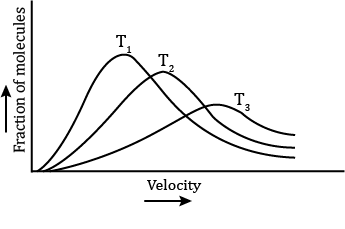
\includegraphics[height=.25\textheight]{res/maxwell.png}
  \captionsetup{justification=centering,margin=3cm}
  \caption{Phân bố Maxwell, được dùng trong động học chất khí để mô tả vận tốc
  các phân tử khí.}
\end{figure}
\end{frame}

\begin{frame}{Mô hình hóa quần thể bằng lý thuyết xác suất}
  Ta có một số các giả định như sau:
  \begin{itemize}
  \item Khi khởi tạo quần thể, ta thu được một phân bố quần thể là một phân bố
    liên tục và luôn dương.
  \end{itemize}

  Khi quần thể của ta là vô cùng lớn, ta có thể coi quần thể là một phân bố xác
  suất. Các cá thể có nhiều cá thể giống mình sẽ tương ứng với các giá trị mà tại đó
  hàm mật độ xác suất (PDF) có giá trị lớn và ngược lại.

  Tại thế hệ thứ \( g \),ta chia quần thể chung \( P^{g} \) với PDF \( p^{g}(x)
  \) thành các quần thể con \( P_{k}^{g} \), gồm có các cá thể có loài \( k \)
  (skill factor là \( k \)). Quần thể con \( P^{g}_{k} \) có hàm mật độ xác suất
  \( p^{g}_{k}(x) \):
\[
  p^{g}(x) = w_{1}p^{g}_{1}(x) + 
w_{2}p^{g}_{2}(x) + 
\ldots +
w_{T}p^{g}_{T}(x)
,\]
với các trọng số \( w_{i} \) là tỉ lệ số loài của quần thể con trong quần thể
chung: \( w_{k} = \frac{|P_{k}|}{|P|} \).
\end{frame}

\begin{frame}{Mô hình hóa quần thể bằng lý thuyết xác suất}
  Bali \textit{et al.} chứng minh được công thức sau, cho biết PDF của quần thể
  gồm các cá thể con loài \( k \) được sinh ra cũng là một tổ hợp tuyến tính của
  các hàm \( p_{1}^{g}, p_{2}^{g}, \ldots, p_{T}^{g} \):
  \begin{align*}
    q^{g}_{k}(x) &= \sum_{i = 1}^{T} \alpha_{i}^{g} p_{i}^{g}(x)\\
    \alpha_{k} &= 1- \frac{(T-1)rmp}{2T}\\
    \alpha_{j} &= \frac{rmp}{2T}, \forall j \neq  k\\
  .\end{align*}
\end{frame}
\begin{frame}{Mô hình hóa quần thể bằng lý thuyết xác suất}
  Quá trình chọn lọc cũng có thể được mô hình bằng công thức sau:
  \[
    p^{g+1}_{k}(x) = \begin{cases}
      \frac{q^{g}_{k}(x)}{\theta }, &\text{ nếu }f_{k}(x) \ge \beta^{g}_{k}\\
      0, & \text{ nếu ngược lại}
    \end{cases}
  ,\] 
  với \( \beta^{g}_{k} \) là ngưỡng chọn lọc của bài toán \( k \) trong thế hệ
  \( g \), \( \theta \) là tỷ lệ các cá thể được chọn:
  \[
    \int _{f_{k}(x) \ge \beta^{g}_{k}} q^{g}_{k}(x) = \theta
  .\] 
\end{frame}
\begin{frame}{Mô hình hóa quần thể bằng lý thuyết xác suất}
  Mặt khác, ta lại có:
  \begin{align*}
    \theta = \int _{f_{k}(x) \ge \beta^{g+1}_{k}} q^{g+1}_{k}(x)dx &= \alpha_{k}\int
    _{f_{k}(x) \ge \beta^{g+1}_{k}} p^{g+1}_{k}(x)dx + \underbrace{\sum_{\substack{i = 1\\i \neq    k}}^{T}\alpha_{i}\int
  _{f_{k}(x) \ge \beta^{g+1}_{k}} p^{g+1}_{i}(x)}_{\ge 0} \\
&\ge \alpha_{k} \int_{f_{k}(x) \ge B} p^{g+1}_{k}(x)dx, (B = \max
  \{\beta^{g}_{k}, \beta^{g+1}_{k}\}  )
  .\end{align*}

  Nếu \( \alpha_{k} > \theta \), thì tích phân cuối phải nhỏ hơn \( 1 \). Mà
  do \( \int _{f_{k}(x) \ge \beta^{g+1}_{k}} p^{g+1}_{k}(x) = 1 \) nên bắt buộc
  \( B < \beta^{g+1}_{k} \iff \boxed{\beta^{g}_{k} < \beta^{g+1}_{k}} \)
\end{frame}

\begin{frame}{Mô hình hóa quần thể bằng lý thuyết xác suất}
  Do \( \beta^{g}_{k} \) tăng (theo \( g \)) nên dãy này hội tụ tại \( f'_{k}
  \). Nếu giới hạn này lớn hơn giá trị tối ưu của hàm \( f_{k} \), ta có thể
  chứng minh sự mâu thuẫn bằng cách sử dụng đánh giá sau:
  \[
    p^{g}_{k}(x) \ge \left( \frac{\alpha_{k}}{\theta} \right) ^{g} p^{0}_{k}(x),
    \forall x: f_{k}(x) > f'_{k}
  ,\] suy được từ đánh giá tích phân.

  Do đó, cho \( g \to +\infty \), hàm \( p_{k} \) hội tụ đến vô cùng trên một
  đoạn có độ đo khác \( 0 \) (tập \( H \) gồm các điểm \( x \) thỏa mãn \(
  f_{k}(x) > f'_{k}\)), nên ta có:
  \[
    \lim_{g \to \infty} \int_{H} p^{g}_{k}(x) = +\infty
  .\] 
  Giới hạn này mâu thuẫn với việc các hàm \( p^{g}_{k} \) là các hàm mật độ xác
  suất. Do đó, \( \beta^{g}_{k} \) hội tụ tới giá trị tối ưu của hàm \(
  f_{k} \), nên thuật toán luôn luôn hội tụ cho bài toán \( k \) nếu có điều
  kiện \( \alpha_{k} > \theta \).
\end{frame}
\begin{frame}{Mô hình hóa quần thể bằng lý thuyết xác suất}
  Mặt khác, do \( \alpha_{k} = 1 - \frac{(T-1)rmp}{2T} > \frac{1}{2} \), nên
  thuật toán luôn luôn hội tụ (theo lý thuyết) nếu trong bước chọn lọc ta chỉ
  giữ lấy ít hơn một nửa số cá thể.

  Hơn nữa, từ những đánh giá trên, Bali \textit{et al.} còn đánh giá được
  rằng tốc độ hội tụ của thuật toán càng nhanh nếu phân phối \( q^{g}_{k} \)
  càng giống với \( p^{g}_{k} \). Do đó, theo đánh giá này, nếu \( rmp = 0
  \), \( \alpha_{k} = 1 \) và \( \alpha_{j} = 0 \) với mọi \( j \neq k \), thì
  \( p^{g}_{k} = q^{g}_{k} \) và theo lý thuyết thuật toán sẽ hội tụ nhanh nhất.
\end{frame}
% subsection Khảo sát tính hội tụ của thuật toán MFEA (end)

\subsection{Điều chỉnh xác suất lai ghép khác loài} % (fold)
\label{sub:Điều chỉnh xác suất lai ghép khác loài}

\begin{frame}{Ma trận xác suất lai ghép}
Trong phần trước, ta thấy rằng \( rmp \) càng làm cho phân phối của quần thể con
giống với quần thể cha mẹ thì quá trình chuyển giao tri thức càng hiệu quả. Với
ý tưởng này, ta có thể thực hiện cập nhật ma trận xác suất lai ghép một cách tự
động.

Trước hết, ta chuyển từ sử dụng một số \( rmp \) sang sử dụng ma trận \( RMP \):
\[
  RMP = \begin{bmatrix}
    RMP_{1, 1} & RMP_{1, 2} & \ldots \\
    RMP_{2,1} & RMP_{2,2} & \ldots \\
    \vdots & \vdots & \ddots
  \end{bmatrix} 
.\]
Ở đây, \( RMP_{i,j} \) là xác suất lai ghép giữa loài \( i \) và loài \( j \).
Vì trong thuật toán gốc ta luôn cho phép lai ghép cùng loài, nên \( RMP_{i,i} =
1, \forall i=\overline{1,T}\).

Ta không làm như thế này ở thuật toán gốc là vì việc sử dụng một ma trận RMP như
thế này sẽ sinh ra quá nhiều tham số. Do những tham số này sẽ được cập nhật tự
động trong thuật toán này, sử dụng nhiều tham số không còn là một vấn đề nữa.
\end{frame}


\begin{frame}{Cập nhật xác suất lai ghép}
  Để đo lường sự tương đồng giữa hai phân phối của quần thể con (có hàm PDF là
  \( q_{k}^{g}(x) \)) và quần thể cha mẹ (có hàm PDF là \( p_{k}^{g}(x) \)), ta
  sử dụng độ phân kỳ Kullback-Leibler:
  \[
    KL(P^{g}_{k}\mid \mid Q^{g}_{k}) = \int_{X} p^{g}_{k}(x) \log
    \frac{p^{g}_{k}(x)}{q^{g}_{k}(x)} dx
  .\] 
  Trong đó, \( X \) là không gian bao gồm mọi cá thể hợp lệ của bài toán thứ \(
  k\).

  Giá trị này thường được coi là một độ đo giữa hai phân phối. Nó càng nhỏ nếu
  hai phân phối càng gần nhau và ngược lại. Do đó, ta sẽ cập nhật \( RMP \) để
  làm cho giá trị này đạt giá trị nhỏ nhất.
\end{frame}

\begin{frame}{Cập nhật xác suất lai ghép}
  Đầu tiên, ta thấy:
  \[
    KL(P^{g}_{k}\mid \mid Q^{g}_{k}) = \underbrace{\int_{X} p^{g}_{k}(x) \log
    p^{g}_{k}(x)dx}_{\text{const}} - \int_{X} p^{g}_{k}(x) \log q^{g}_{k}(x)dx
  .\] 

  Do đó, ta sẽ cần tối đa tích phân \( \int_{X} p^{g}_{k}(x) \log q^{g}_{k}(x)dx
  \). Tích phân này lại chính là kì vọng của biến ngẫu nhiên \( \log
  q^{g}_{k}(P^{g}_{k}) \).

  Sau khi rởi rạc hóa, ta đưa bài toán ban đầu thành:
  \[
    \max c_{k}(RMP) = \sum_{x \in P^{g}_{k}} \log q^{g}_{k}(x)
  .\]
\end{frame}

\begin{frame}{Cập nhật xác suất lai ghép}
  Do ta có \( T \) hàm mục tiêu cho bài toán tối ưu \( RMP \), nên ta cần đưa
  bài toán đa mục tiêu này về bài toán đơn mục tiêu:
  \[
    \max c(RMP) = \sum_{k = 1}^{T} c_{k}(RMP) = \sum_{k = 1}^{T} \sum_{x \in
    P^{g}_{k}} \log q^{g}_{k}(x)
  .\] 
  Công thức của hàm \( q^{g}_{k} \) được tính qua hàm \( p^{g}_{k} \). Hàm này
  sẽ được ước tính tử quần thể \( P^{g}_{k} \). Ngoài ra, công thức của các hệ
  số \( \alpha_{k} \) cũng thay đổi do biến \( RMP \) là một ma trận:
  \begin{gather*}
    \alpha_{j} = \frac{RMP_{k,j}}{2T}, \forall  j \neq k\\
    \alpha_{k} = 1 - \frac{1}{2T}\sum_{j \neq  k} RMP_{k, j}\\
    q^{g}_{k}(x) = \sum_{j = 1}^{T} \alpha_{j}p^{g}_{j}(x)
  .\end{gather*}
\end{frame}

\begin{frame}{Cập nhật xác suất lai ghép}
  Vậy, quá trình cập nhật ma trận xác suất lai ghép \( RMP \) có thể được tóm
  tắt bằng các bước sau:
  \begin{itemize}
  \item Ước lượng các quần thể con \( P^{g}_{k} \) bằng các phân phối liên tục có
    hàm mật độ là \( p^{g}_{k} \).
  \item Từ các hàm mật độ sự phân bố  các cá thể cha mẹ \( p^{g}_{k} \), tính
    hàm mật độ cho các cá thể con \( q^{g}_{k} \).
  \item Thay các hàm \( q^{g}_{k} \) vào bài toán tối ưu biến \( RMP \) và giải
    bài toán này.
  \end{itemize}

  Thuật toán MFEA có sử dụng thêm phương pháp cập nhật xác suất lai ghép này
  được gọi là thuật toán \textbf{MFEA-II}.
\end{frame}
% subsection Điều chỉnh xác suất lai ghép khác loài (end)

% section Thuật toán Tiến hóa Đa yếu tố (MFEA) (end)

\section{Các framework tiến hóa đa nhiệm} % (fold)
\label{sec:Các framework tiến hóa đa nhiệm}

\subsection{Mô hình chung} % (fold)
\label{sub:Mô hình chung}

\begin{frame}{Mô hình chung}
Nhắc lại, thuật toán MFEA được phát triển từ cách chuyển bài toán đa
nhiệm:
\begin{align*}
  \min &\, f_{1}(x_{1}), f_{2}(x_{2}), \ldots , f_{T}(x_{T})\\
  \text{subject to}\, &x_{1} \in X_{1}, x_{2} \in X_{2},
  \ldots , x_{T} \in X_{T}.
\end{align*}
Thành bài toán đơn nhiệm:
\begin{align*}
  \min &\, f(x) = f_{1}(x_{1})+ f_{2}(x_{2})+ \ldots +
  f_{T}(x_{T})\\
  \text{subject to}\, &x = (x_{1}, x_{2}, \ldots, x_{T}) \in X_{1} \times  X_{2}
  \times  \ldots  \times X_{T}.
\end{align*}
Ở đây ta sẽ tiếp cận theo hướng ngây thơ còn lại: chia bài toán đa nhiệm thành
\( T \) bài toán đơn nhiệm và phát triển lên để thu được các \textbf{framework
tiến hóa đa nhiệm}.
\end{frame}

\begin{frame}[fragile]
\frametitle{Mô hình chung}
Như đã nói ở phần mở đầu về tiến hóa đa nhiệm, ta can thiệp vào quá trình
chạy thuật toán để thực hiện chuyển giao tri thức:
\begin{minted}[fontsize=\footnotesize]{python}
def mfo():
  while True:
    # nếu vòng lặp này thực hiện chuyển giao tri thức
    if culture_tranmission():
      yield do_culture_tranmission() # thực hiện chuyển giao tri thức
    else:
      # nếu không chuyển giao, chạy thuật toán đơn nhiệm
      # một cách độc lập cho từng bài toán
      populations = [next(task.ea) for task in tasks]
      # trả lại quần thể
      yield populations
\end{minted}

Ở đây, điều kiện \( \texttt{culture\_tranmission()} \) có thể được cài đặt tùy ý.
Chẳng hạn như ta có thể cho chuyển giao tri thức cứ \( \alpha \) thế hệ một lần
(\( \texttt{gen \% alpha == 0} \)),
hoặc dựa vào xác suất thông qua một biến ngẫu nhiên (\( \texttt{random.random()
< p} \)).
\end{frame}

\begin{frame}[fragile]
\frametitle{Mô hình chung}
Ta cũng có thể cho điều kiện chuyển giao tri thức phụ thuộc vào từng bài toán:
\begin{minted}[fontsize=\footnotesize]{python}
def mfo():
  while True:
    populations = []
    for task in tasks:
      if culture_tranmission(task):
        populations += [do_culture_tranmission(task)]
      else:
        populations += [next(task.ea)]
    yield populations
\end{minted}

Có thể thấy, cách làm hiện tại tách biệt giữa việc chuyển giao tri thức với chạy
một thuật toán tiến hóa đơn nhiệm, nghĩa là ta có thể sử dụng các thuật giải
khác nhau cho từng bài toán.
\end{frame}

\begin{frame}[fragile]
\frametitle{Mô hình chung}
  Một cách cụ thể để thực hiện chuyển giao tri thức là chuyển giao trực tiếp các
  cá thể từ các quần thể khác sang quần thể của bài toán đang xét:
  \begin{minted}{python}
import random

def do_culture_tranmission(task):
  # quần thể gồm mọi cá thể trừ các cá thể của bài toán đang xét
  pop_all = [x for transfer_task in tasks if transfer_task != task
               for x in task.population]
  # chọn lấy 100 cá thể ngẫu nhiên từ `pop_all`
  task.population += random.sample(pop_all, 100)
  return selction(task) # thực hiện chọn lọc
  \end{minted}
\end{frame}

\begin{frame}[fragile]
\frametitle{Mô hình chung}
Ngoài cách chọn giữa chuyển giao tri thức hoặc chạy một vòng lặp đơn nhiệm, ta
cũng có thể can thiệp vào quá trình chuyển giao tri thức bằng cách thêm các cá
thể con sinh ra từ lai ghép khác loài vào thế hệ con sinh ra từ thuật toán đơn
nhiệm.
\begin{minted}[fontsize=\footnotesize]{python}
def mfo():
  while True:
    populations = []
    for task in tasks:
      offsprings = reproduction(task) # lai ghép cùng loài
      for transfer_task in tasks:
        if task != transfer_task:
          # tính số lượng cá thể con sinh ra từ lai ghép khác loài
          num_offsprings = int(rmp * len(offsprings))
          # thực hiện lai ghép khác loài, thêm các 
          # cá thể con này vào mảng `offspring`
          offsprings += interspecies_mating(task, transfer_task, num_offsprings)
      task.population += offsprings
      populations += selection(task.population)
    yield populations
\end{minted}
\end{frame}

\begin{frame}[fragile]
\frametitle{Mô hình chung}
Ở đây, xác suất chuyển giao khác loài, biến \( rmp \), không nhất thiết phải
giống nhau cho mọi cặp bài toán. Ta hoàn toàn thay thế nó bằng một ma trận \(
RMP \), mã giả trên sử dụng một tham số chỉ để làm thuật toán dễ đọc hơn.

Khi các xác suất \( rmp \) khác nhau và phụ thuộc vào từng cặp bài toán, ta có
thể chỉ thực hiện lai ghép khác loài với bài toán \( \texttt{transfer\_task}
\) có xác suất này lớn nhất.

Trong thuật toán EBS của Liaw và Ting, ngoài việc chỉ chuyển giao với bài toán
có xác suất \( rmp \) lớn nhất, còn có một khác biệt nhỏ là các cá thể con
sinh ra từ lai ghép khác loài sẽ thay thế các cá thể cuối của mảng \(
\texttt{offsprings} \):
\begin{minted}{python}
# thay `num_offsprings` phần tử cuối của mảng `offspring`
# bởi kết quả trả lại ở vế phải
offsprings[-num_offsprings:] = interspecies_mating(task, transfer_task,
                                                   num_offsprings)
\end{minted}
\end{frame}
% subsection Mô hình chung (end)

\subsection{Chọn cá thể chuyển giao bằng phát hiện bất thường} % (fold)
\label{sub:Chọn cá thể chuyển giao bằng phát hiện bất thường}

\begin{frame}{Phát hiện bất thường}
  Phát hiện bất thường là một cách phân loại dữ liệu trong học máy. Việc phân
  biệt giữa các dữ liệu bình thường và bất thường là vô cùng quan trọng, vì các
  dữ liệu bất thường không những không có đủ để có thể được xử lý như các dữ
  liệu bình thường, mà nó còn làm lệch đi các giá trị được xử lý.

  Trong tiến hóa đa nhiệm, ta có thể coi các bất thường là những cá thể có thể
  chuyển giao nhiều thông tin di truyền xấu, nên ta cần hạn chế lai ghép khác
  loài với các cá thể bất thường.

  Để phát hiện sự bất thường, cách đơn giản nhất là sử dụng một phân phối xác
  suất với hàm mật độ \( f(x) \) cho dữ liệu. Những giá trị \( x \) có \( f(x)
  \) quá thấp sẽ bị coi là dữ liệu bất thường. Phân phối xác suất hay được sử
  dụng ở đây chính là phân phối chuẩn nhiều biến \( \mathcal{N}(\mu, \Sigma) \).
\end{frame}

\begin{frame}{Chọn lọc cá thể chuyển giao dựa trên phát hiện bất thường}
Sử dụng phương pháp phát hiện bất thường, khi ta chọn các cá thể để lai ghép
khác loài, ta sẽ ưu tiên chọn những cá thể "bình thường nhất", nghĩa là các cá
thể \( x \) sao cho \( f(x) \) lớn nhất.

Thuật toán MTEA-AD của Wang \textit{et al.} chọn ra \( T_{k} \) là tập gồm có \(
\varepsilon_{k} (|P| - |P_{k}|) \) cá thể
có \( f(x) \) lớn nhất từ quần thể \( P \setminus P_{k} \), với \( P_{k} \) là
quần thể của bài toán đang xét và \( P \) là quần thể tổng gồm tất cả các cá
thể. Tham số \( \varepsilon_{k} \) sẽ được cập nhật dựa vào độ hiệu quả của chuyển
giao tri thức:
\[
  \varepsilon_{k} = \frac{s_{k}}{m_{k}}
,\]

với \( s_{k} \) và \( m_{k} \) là số lượng cá thể trong và ngoài \( T_{k} \)
được giữ lại sau bước chọn lọc.
\end{frame}

\begin{frame}[fragile]
\frametitle{Chọn lọc cá thể chuyển giao dựa trên phát hiện bất thường}
  Thuật toán MTEA-AD thực hiện chuyển giao tri thức như sau:
\begin{minted}[fontsize=\footnotesize]{python}
def mtea_ad():
  while True:
    populations = []
    for task in tasks:
      offsprings = reproduction(task) # tạo thế hệ con
      transfers = ad_select(task) # chọn T_k
      # thêm vào quần thể và chọn lọc
      task.population += offsprings + transfers 
      populations += [selection(task)]
      # sau đó, cập nhật giá trị epsilon
      update_epsilon(task)
    yield populations
\end{minted}
\end{frame}

% subsection Chọn cá thể chuyển giao bằng phát hiện bất thường (end)

\subsection{Cập nhật xác suất chuyển giao dựa trên quan hệ sinh học} % (fold)
\label{sub:Cập nhật xác suất chuyển giao dựa trên quan hệ sinh học}

\begin{frame}{Mối quan hệ các loài trong sinh học}
Trong hệ sinh thái gồm rất nhiều loài sinh vật tương tác với nhau, các nhà sinh
học đã đưa ra các loại mối quan hệ giữa hai cá thể khác loài \( a \) và \( b \),
gồm có:
\begin{itemize}
\item Hỗ trợ (M): \( a \) có lợi với \( b \) và ngược lại.
\item Hội sinh (O): \( a \) có lợi với \( b \), \( b \) không có lợi và không có
  hại với \( a \).
\item Ký sinh (P): \( a \) có lợi với \( b \) nhưng \( b \) có hại với \( a \).
\item Trung lập (N): \( a \) không có hại, không có lợi với \( b \) và ngược lại.
\item Chống cộng sinh (A): \( a \) không có lợi, không có hại với \( b \), nhưng \(
  b \) có hại với \( a \).
\item Cạnh tranh (C): \( a \) có hại với \( b \) và ngược lại.
\end{itemize}

Chú ý ở dây, các mối quan hệ hội sinh, ký sinh và chống cộng sinh là không đối
xứng.
\end{frame}

\begin{frame}{Mối quan hệ các cá thể trong sinh học}
Các định nghĩa trên có thể được viết lại dưới dạng các mối quan hệ giữa các loài
trong một giải thuật tiến hóa đa nhiệm. Chẳng hạn, mối quan hệ giữa
loài \( \tau_{1} \) và \( \tau_{2} \) \textbf{đối với một cá thể} \( x \) là
hỗ trợ nếu \( x \) đều có lợi với \( \tau_{1} \) và \( \tau_{2} \).

Bằng cách đếm số cá thể \( x \) thoả mãn điều kiện trên, ta có thể ước chừng
được một cách tương đối rằng hai loài \( \tau_{1} \) và \( \tau_{2}  \) hỗ trợ
nhau nhiều hay ít. So sánh số này với các số đếm thu được cho các mối quan hệ
khác, ta có thể đánh giá được tính hiệu quả của việc chuyển giao tri thức như
sau:
\[
  r = \frac{M + O + P}{M + O + P + A + C + N}
.\] 
Ở đây, các biến in hoa là số đếm cho các mối quan hệ tương ứng. \( M, O, P \)
tượng trưng cho mối quan hệ hỗ trợ, hội sinh và ký sinh, là các mối quan hệ có
ảnh hưởng tốt cho việc chuyển giao tri thức (từ loài \( \tau_{1} \) sang \(
\tau_{2}\), không nhất thiết ngược lại).
\end{frame}

\begin{frame}{Mối quan hệ các cá thể trong sinh học}
  Tuy nhiên, để xác định các mối quan hệ này, ta cần định nghĩa như thế nào là
  có lợi và có hại.
  
  Liaw và Ting định nghĩa hai mối quan hệ này như sau:
  \begin{itemize}
  \item Có lợi: \( a \) có lợi với loài \( \tau \) nếu \( a \) nằm
    trong\footnote{Do \( a \) không có loài \( \tau \) nên một cách chính xác
    hơn để định nghĩa là \( a \) tốt hơn (hoặc tốt bằng) cá thể cuối cùng thuộc top \(
  \mathcal{B}\% \) của loài này.} top \(
    \mathcal{B}\%\) các cá thể tốt nhất của loài này.
  \item Có hại: \( a \) có hại với loài \( \tau \) nếu \( a \) nằm trong top \(
    \mathcal{H}\% \) các cá thể kém nhất của loài này.
  \end{itemize}

  Các tham số \( \mathcal{B} \) và \( \mathcal{H} \) được gọi là hệ số có lợi và
  hệ số có hại.
\end{frame}
\begin{frame}[fragile]
\frametitle{Thuật toán EBS}
\begin{minted}[fontsize=\footnotesize]{python}
def ebs():
  populations = []
  for task in tasks:
    offsprings[task] = reproduce(task.ea)
  for task in tasks:
    # tìm bài toán chuyển giao tốt nhất
    transfer_task = max(tasks, key=r[task])
    num_offsprings = int(r[task][transfer_task] * len(offsprings))
    offsprings[task][-num_offsprings:] = offsprings[transfer_task][:num_offsprings]
    task.population += offsprings[task]
    populations += [selection(task.ea)]
    update_rate() # cập nhật các giá trị r[t1][t2]
  yield populations
\end{minted}

Ở đây, hiệu quả chuyển giao (\( \texttt{r[task][transfer\_task]} \)) được sử
dụng để chọn ra bài toán tốt nhất để chuyển giao và số lượng cá thể con được
chuyển giao. Ta hoàn toàn cũng có thể trực tiếp chuyển giao cá thể cha mẹ thay
vì chuyển giao các cá thể con.
\end{frame}
% subsection Cập nhật xác suất chuyển giao dựa trên quan hệ sinh học (end)

\subsection{Cập nhật xác suất chuyển giao dựa trên nhật ký} % (fold)
\label{sub:Cập nhật xác suất chuyển giao dựa trên nhật ký}

\begin{frame}{Nhật ký và so sánh nhật ký}
Nhật ký của một loài là một tập các cá thể của loài này xuyên suốt quá trình
thuật toán được chạy. Nó bao gồm các cá thể của thế hệ hiện tại và các thế hệ
trước đó của loài.

Ý tưởng của cách cập nhật xác suất này là so sánh giữa các nhật ký. Cách làm của
Chen \textit{et al.} là sử dụng phân phối chuẩn nhiều biến và tính độ phân kỳ
Kullback-Leibler giữa các phân phối. Chẳng hạn, với hai quần thể \( P_{1} \) và
\( P_{2} \), ta tính kì vọng \( \mu_{1}, \mu_{2} \) và ma trận hiệp phương sai
\( \Sigma_{1}, \Sigma_{2} \). Khi đó, độ phân kỳ giữa hai phân phối xác suất
tượng trưng cho hai quần thể là:
\[
  D_{KL}(P_{1}\mid \mid P_{2}) = \frac{1}{2} \left(
  \operatorname{tr}(\Sigma_{2}^{-1}\Sigma_{1}) +
(\mu_{2}-\mu_{1})^{T}\Sigma_{1}^{-1}(\mu_{2}-\mu_{1}) + \log
\frac{\operatorname{det} \Sigma_{2}}{\operatorname{det} \Sigma_{1}} - D \right) 
.\] 
Do độ phân kỳ Kullback-Leibler không đối xứng, nên ta cần đối xứng hóa như sau:
\[
  \operatorname{Sim}(P_{1}, P_{2}) = \frac{1}{2} \left( D_{KL}(P_{1}\mid \mid
  P_{2}) + D_{KL}(P_{2}\mid \mid P_{1}) \right) 
.\] 
\end{frame}

\begin{frame}[fragile]
\frametitle{Nhật ký và so sánh nhật ký}
  Sau mỗi thế hệ, ta sẽ tiến hành cập nhật nhật ký. Để nhật ký chứa cả các cá
  thể từ thế hệ hiện tại và các thế hệ trước, chẳng hạn, thuật toán MaTEA thực
  hiện như sau:
  \begin{minted}[fontsize=\footnotesize]{python}
import random

def update_archive(task):
  for x in task.population: # lặp với mọi cá thể
    # với xác suất `update_rate`, cho cá thể vào nhật ký
    if random.random() < update_rate: 
      if task.archive.full(): # nếu nhệt ký đầy, thay thế cá thể ngẫu nhiên
        i = random.choice(range(len(task.archive)))
        task.archive[i] = x
      else: # nếu chưa đầy thì thêm vào nhật ký
        task.archive += [x]
  \end{minted}
\end{frame}
\begin{frame}{Adaptive Reward Strategy}
  Chỉ so sánh giữa các nhật ký để tính xác suất chuyển giao sẽ không phân biệt
  được giữa chuyển giao tri thức tốt và tri thức xấu. Do đó, ta sử dụng thêm một
  biến \( R \) cho mỗi cặp bài toán để đánh giá tính tốt xấu của việc chuyển
  giao tri thức. Biến này sẽ được tăng nếu như việc chuyển giao là tốt, bị giảm
  nếu chuyển giao là xấu:
  \[
    R \coloneqq \begin{cases}
      R / \lambda, &\text{ nếu chuyển giao tri thức tốt } \\
      R \cdot \lambda, &\text{ nếu chuyển giao tri thức xấu }
    \end{cases}
  .\] 
  \( \lambda \) là một hằng số trong \( [0, 1] \).

  Để quyết định chuyển giao là tốt hay xấu, ta có thể so sánh giữa các cá thể
  trong quần thể của bài toán với các cá thể chuyển giao. Thuật toán MaTEA của
  Chen \textit{et al.} so sánh \( p_{best} \), cá thể tốt nhất của quần thể bài
  toán với các cá thể \( o \) sinh ra từ lai ghép chuyển giao tri thức. Chuyển
  giao tri thức được coi là xấu nếu \( p_{best} \) tốt hơn mọi \( o \) và là tốt
  nếu ngược lại.
\end{frame}

\begin{frame}{Adaptive Reward Strategy}
  Lấy ý tưởng từ Reinforcement Learning, với mỗi cặp bài toán, ta sẽ có một biến
  điểm là \( score \). Biến này sẽ được cập nhật như sau:
  \[
    score \coloneqq \rho \cdot score + \frac{R}{\log Sim(P_{1}, P_{2})}
  .\] 
  \( \rho \) là một hằng số trong \( [0, 1] \).

  Các biến điểm này có thể được sử dụng để so sánh hiệu quả chuyển giao tri thức
  giữa các bài toán với nhau. Tuy nhiên, biến này chỉ mang tính tương đối (chỉ
  có ý nghĩa khi được so sánh với các biến điểm của các cặp bài toán khác).

  Trong thuật toán MaTEA, các biến điểm này được sử dụng làm trọng số để chọn
  bài toán chuyển giao theo cách Roulette Wheel Selection, nhưng nói chung là
  ta cũng có thể sử dụng các cách khác. Cách làm như thế này được Chen
  \textit{et al.} gọi là \textbf{Adaptive Reward Strategy}.
\end{frame}

\begin{frame}[fragile]
\frametitle{Thuật toán MaTEA}
\begin{minted}[fontsize=\footnotesize]{python}
def matea():
  while True:
    populations = []
    for task in tasks:
      if random.random() < alpha:
        # chạy một vòng lặp đơn nhiệm
        populations += [next(task.ea)]
      else:
        # chọn bài toán chuyển giao tri thức
        transfer_task = roulette_select(tasks, key=score[task])
        # lai ghép chuyển giao tri thức
        offsprings = knowledge_transfer_crossover(task, transfer_task)
        task.population += offsprings
        population += [selection(task)]
        update_scores(task, transfer_task) # cập nhật score[task][transfer_task]
      update_archive(task) # cập nhật nhật ký
\end{minted}
\end{frame}
% subsection Cập nhật xác suất chuyển giao dựa trên nhật ký (end)

% section Các framework tiến hóa đa nhiệm (end)


\section{Tài liệu tham khảo}
\begin{frame}[allowframebreaks]{Tài liệu tham khảo}
    \nocite{*}
    \bibliographystyle{plainnat}
    \bibliography{main.refs.bib}
\end{frame}

\begin{frame}{~}
    % \Large \color{hustred}{Cảm ơn mọi người đã chú ý lắng nghe!}
\end{frame}

\end{document}
